\chapter{Turbo Muon}

\section{On the convergence of \turbomuon}
\subsection{Link with norm  constrained steepest descent}
\label{ap:proof_convergence}
% \iffalse
    In this section, we build upon the work of \cite{bernstein2024oldoptimizernewnorm}, as they show that Muon's update (without accumulation) solves a steepest descent direction in a $\ell_2 \rightarrow \ell_2$ induced operator norm.
    As a starting point, we define how the norm induced by our preconditioning differs from the original one. We show in \cref{supp:descent_proof}
    that preconditioning does not bias the overall optimization process.
    
    \hfill
    
    Following \cite{bernstein2024oldoptimizernewnorm}, we formulate the steepest descent update using a penalized objective, which is equivalent to the constrained formulation for a specific step size $\eta$, i.e.:
    
    \begin{equation}
        \arg \min_{\Delta W \in \mathbb{R}^{m \times n}} \left[ \langle G, \Delta W \rangle + \frac{\lambda}{2} \| \Delta W\|_{\alpha \rightarrow \beta}^2 \right],
    \label{eq:steepest_descent}
    \end{equation}
    
    \noindent where $\langle \cdot , \cdot \rangle$ denotes the Frobenius inner product. For any matrix $M \in \mathbb{R}^{m \times n}$, and normed spaces $(\mathbb{R}^{d_\mathrm{in}}, \| \cdot \|_\alpha)$ and $(\mathbb{R}^{d_\mathrm{out}}, \| \cdot \|_\beta)$, the ``$\alpha$ to $\beta$'', we recall the induced operator norm as:
    
    \begin{equation}
        \| M \|_{\alpha \rightarrow \beta} = \max_{x \in \mathbb{R}^{d_\mathrm{in}}} \frac{\| M x \|_\beta}{\| x \|_\alpha}.
    \end{equation}
    
    \noindent Importantly, as explicited in Proposition 5 of \cite{bernstein2024oldoptimizernewnorm}. When $\alpha = 2$ and $\beta = 2$, we have that the solution to Equation~\ref{eq:steepest_descent} is:
    
    
    \begin{equation*}
        \Delta W_{\| \cdot \|_{\ell_2 \rightarrow \ell_2}} = -\eta \operatorname{PolarFactor}(G),
    \end{equation*}
    
    \noindent with $\eta$ the sum of the singular values of $G$ divided by $\lambda$. In this paper, we introduce the \turbomuon update as $\operatorname{PolarFactor}(G S)$. With $S$ the diagonal matrix composed of AOL preconditioning coefficients (previously denoted as $s$), which are strictly positive and bounded in practice. Here we show that this update is the solution of a slightly different steepest descent direction problem formulated using a rescaled norm.
% \fi
    % As a reminder of the \cref{prop:convergence}:
    
    % \begin{proposition}[\turbomuon Steepest Descent]
    %     Given any diagonal matrix $S\in \mathbb{R}_{>0}^{n \times n}$ (strictly positive)
    %     %\franck{j'ai pas mis la condition bounded enties est-ce que ce n'est pas evident sur une matrice de taille finie?}), 
    %     and for any gradient matrix $G \in \mathbb{R}^{m \times n}_{\setminus 0}$ 
    %     , and any sharpness $\lambda > 0$, consider the problem:
        
    %     \begin{equation}
    %     \begin{aligned}
    %         & \arg \min_{\Delta W \in \mathbb{R}^{m \times n}} \left[  \langle G, \Delta W \rangle_F + \frac{\lambda}{2} \| \Delta W \|_{\ell_2 \rightarrow S}^2 \right] \quad
    %          \text{with} \ \| M \|_{\ell_2 \rightarrow S} := \sup_{x \in \mathbb{R}^{n}_{\setminus 0}} \frac{\| M S^{-1} x \|_2}{\| x\|_2}.
    %     \end{aligned}
    %     \end{equation}
    % %\franck{vu la position de $\alpha$ et $\beta$, j'ai inversé S et $\ell_2$ }
    %     \noindent This problem is solved with a step size $\eta = \frac{1}{\lambda} \operatorname{tr}(\Sigma_{GS})$, with $GS=U \Sigma_{GS} V^\top$ the SVD decomposition of $GS$, with $U$ and $V$ unitary,  and an update:
    
    %     \begin{equation}
    %         \Delta W_{\| \cdot \|_{\ell_2 \rightarrow S}} = -\eta \operatorname{PolarFactor}(G S),
    %     \end{equation}
    
    %     \noindent This solution is unique if and only if $G$ is of full rank. %We assume $S$ to be a matrix whose diagonal is filled with rescaling values obtained from \cref{eq:aol} (strictly positive and bounded diagonal).
    % \end{proposition}

 % \iffalse
    
    \begin{proposition}[\turbomuon in the Steepest Descent framework]
    For any gradient matrix $G \in \mathbb{R}^{m \times n}_{\setminus 0}$, and any sharpness $\lambda > 0$, consider the problem:
        
        \begin{equation}
        \begin{aligned}
            & \arg \min_{\Delta W \in \mathbb{R}^{m \times n}} \left[  \langle G, \Delta W \rangle_F + \frac{\lambda}{2} \| \Delta W \|_{\ell_2 \rightarrow S}^2 \right] \\
             \text{with} & \ \| M \|_{\ell_2 \rightarrow S} := \sup_{x \in \mathbb{R}^{n}_{\setminus 0}} \frac{\| M S^{-1} x \|_2}{\| x\|_2}.
        \end{aligned}
        \end{equation}
    %\franck{vu la position de $\alpha$ et $\beta$, j'ai inversé S et $\ell_2$ }
        \noindent This problem is solved with a step size $\eta = \frac{1}{\lambda} \operatorname{tr}(\Sigma_{GS})$, with $GS=U \Sigma_{GS} V^\top$ the SVD decomposition of $GS$, with $U$ and $V$ unitary,  and an update:
    
        \begin{equation}
            \Delta W_{\| \cdot \|_{\ell_2 \rightarrow S}} = -\eta \operatorname{PolarFactor}(G S) S,
        \end{equation}
    
        \noindent This solution is unique if and only if $G$ is of full rank. %We assume $S$ to be a matrix whose diagonal is filled with rescaling values obtained from \cref{eq:aol} (strictly positive and bounded diagonal).

    \end{proposition}
% \fi
    
    This proposition with $S$, the diagonal matrix filled with rescaling values obtained from \cref{eq:aol} (strictly positive),  generalizes a scaled variant of \turbomuon as an optimizer that yields steepest descent directions in an induced norm that is dependent on AOL rescalings, as per the framework of \cite{bernstein2024oldoptimizernewnorm}.
    
    \begin{proof}
    Given the problem 
    
        \begin{equation}
        \begin{aligned}
            & \arg \min_{\Delta W \in \mathbb{R}^{m \times n}} \left[  \langle G, \Delta W \rangle_F + \frac{\lambda}{2} \| \Delta W \|_{\ell_2 \rightarrow S}^2 \right] \\
             \text{with} & \ \| M \|_{\ell_2 \rightarrow S} := \sup_{x \in \mathbb{R}^{n}_{\setminus 0}} \frac{\| M S^{-1} x \|_2}{\| x\|_2}.
        \end{aligned}
        \end{equation}

    By setting $\Delta W' = \Delta W S^{-1}$, we have 
$\| \Delta W \|_{\ell_2 \rightarrow S}^2 = \| \Delta W' \|_{\ell_2 \rightarrow \ell_2}^2$.

Besides using the cyclic property of the trace along with the symmetry of $S$, the inner Frobenius product on the left-hand side of this expression can be modified by:
    \begin{equation}
    \label{eq:frobprod}
    \langle G, \Delta W  \rangle_F = \langle G, \Delta W' S  \rangle_F = \langle G S, \Delta W' \rangle_F
    \end{equation}

    The problem is thus equivalent to minimizing:
    
    \begin{equation}
        \arg \min_{\Delta W' \in \mathbb{R}^{m \times n}} \left[ \langle GS, \Delta W' \rangle + \frac{\lambda}{2} \| \Delta W'\|_{2 \rightarrow 2}^2 \right] 
    \end{equation}
    
    From Proposition 5 of \cite{bernstein2024oldoptimizernewnorm}, the solution of this problem is given by:
    
    
    \begin{equation}
       \Delta W' = - \eta \operatorname{PolarFactor}(GS)
    \end{equation}
    with a step size $\eta = \frac{1}{\lambda} \operatorname{tr}(\Sigma_{GS})$.
    \begin{equation}
       \Delta W = \Delta W' S= - \eta \operatorname{PolarFactor}(GS) S
    \end{equation}

\iffalse
Thus the solution of the problem is 
    \noindent with $X$ of SVD $X = U \Sigma V^\top$ and $\eta = \frac{1}{\lambda} tr (\Sigma)$.
    
    By choosing $X = G S$, this is equivalent to:
    
    \begin{equation}
    \label{eq:polarGS}
        \arg \min_{\Delta W \in \mathbb{R}^{m \times n}} \left[ \langle G S, \Delta W \rangle + \frac{\lambda}{2} \| \Delta W\|_{2 \rightarrow 2}^2 \right] 
        = - \eta \operatorname{PolarFactor}(G S)
    \end{equation}
    
    \noindent First using the cyclic property of the trace along with the symmetry of $S$, the inner Frobenius product on the left-hand side of this expression can be modified by:
    \begin{equation}
    \label{eq:frobprod}
    \langle G S, \Delta W \rangle = \langle G, \Delta W S \rangle
    \end{equation}
    \fi 
    \iffalse    
    \begin{equation}
        \arg \min_{\Delta W \in \mathbb{R}^{m \times n}} \left[ \langle G, \Delta W.S \rangle + \frac{\lambda}{2} \| \Delta W\|_{2 \rightarrow 2}^2 \right] 
        = - \eta \operatorname{PolarFactor}(G S)
    \end{equation}
    \fi
   \iffalse
 
    \noindent The second term  is also equivalent to:
    
    \begin{equation}
    \label{eq:normS}
    \begin{aligned}
       & \| \Delta W\|_{2 \rightarrow 2} = \| \Delta W S \|_{\ell_2 \rightarrow S} \\
        \text{with} & \ \| M \|_{\ell_2 \rightarrow S} := \sup_{x \in \mathbb{R}^{d}} \frac{\| M S^{-1}. x \|_2}{\| x\|_2}.
    \end{aligned}
    \end{equation}
 \fi   
\iffalse
    \begin{equation}
    \begin{aligned}
        \arg \min_{\Delta W \in \mathbb{R}^{m \times n}} &\left[ \langle G, \Delta W.S \rangle + \frac{\lambda}{2} \| \Delta W .S \|_{\ell_2 \rightarrow S}^2 \right] 
        = - \eta \operatorname{PolarFactor}(G S) \\
        &\text{with} \ \| M \|_{\ell_2 \rightarrow S} := \sup_{x \in \mathbb{R}^{d}} \frac{\| M S^{-1}. x \|_2}{\| x\|_2}.
    \end{aligned}
    \end{equation}
\fi
\iffalse

    \noindent by defining $\| M \|_{\ell_2 \rightarrow S}$ the appropriate induced operator norm.

    By a reparametrization with $\Delta W' = \Delta W S$, and introducing \cref{eq:frobprod} and \cref{eq:normS} in \cref{eq:polarGS}, we obtain:
%    Since, in that case, we have: $\| \Delta W \|_{\ell_2 \rightarrow \ell_2}^2 = \| \Delta W . S \|_{\ell_2 \rightarrow S}$. Therefore, we have:
    
    \begin{equation}
        \arg \min_{\Delta W' \in \mathbb{R}^{m \times n}} \left[ \langle G, \Delta W' \rangle + \frac{\lambda}{2} \| \Delta W' \|_{\ell_2 \rightarrow S}^2 \right] = 
        - \eta \operatorname{PolarFactor}(G S),
    \end{equation}
    
    %\noindent by reparametrization with $\Delta W' = \Delta W . S$. 
    To conclude, we have:
    
    \begin{equation}
        \Delta W_{\| \cdot \|_{\ell_2 \rightarrow S}} = - \eta . \operatorname{PolarFactor}(G S)S,
    \end{equation}
    
    \noindent with $\eta = \frac{1}{\lambda} tr (\Sigma_{GS})$, with $GS=U_{GS} \Sigma_{GS} V_{GS}^\top$ the SVD decomposition of $GS$.
    \fi 
    %where we recover the form of 
    The rescaled \turbomuon update is thus close to the solution of a steepest descent framework under the  $\| . \|_{\ell_2 \rightarrow S}$ norm.
    
    \end{proof}

    \paragraph{Discussion:} One main difference between this proof and the update used in \turbomuon is the presence of an extra scaling factor $S$. Applying this scaling vector after the polar factorization would yield an optimizer with dynamics different from Muon's. The exploration of such a novel optimizer is left for future work. 
    
    \subsection{AOL preconditioning cannot lead to Muon divergence}
    \label{supp:descent_proof}
    
        We start by recalling \cref{lem:alignment}:
        

        \begin{lemma*}[Lemma 1]
        \label{lem:alignment2}
            Let $S$ be a diagonal matrix of strictly positive and bounded entries, we have that $\forall \ G \in \mathbb{R}^{m \times n}_{\setminus 0}$:
        
            \begin{equation}
                \langle G, \operatorname{PolarFactor}(GS) \rangle > 0.
            \end{equation}
        
            \noindent Meaning that the projected update recovered by \turbomuon is always ``aligned'' with the raw gradient $G$. Thus, it yields a strict descent direction.
        \end{lemma*}
        
        \begin{proof}
        Write $X:=G S$. By definition of the (left) polar factor,
        \[
            \operatorname{PolarFactor}(X)=X\,(X^\top X)^{-1/2},
        \]
        where $(\cdot)^{-1/2}$ denotes the unique positive–semidefinite inverse square root on the support of $X^\top X$.
        Hence
        \begin{equation*}
        \begin{aligned}
            \langle G,\operatorname{PolarFactor}(G S)\rangle
            &= \operatorname{tr}\!\big(G^\top\,\operatorname{PolarFactor}(X)\big) \\
            &= \operatorname{tr}\!\big(S^{-1}\,X^\top \operatorname{PolarFactor}(X)\big),
        \end{aligned}
        \end{equation*}
        since $G^\top = S^{-1}X^\top$ and $S^{-1}\succ0$ (as per \cref{eq:aol}). Using $X^\top \operatorname{PolarFactor}(X)=X^\top X\,(X^\top X)^{-1/2}=(X^\top X)^{1/2}$, we get
        \[
            \langle G,\operatorname{PolarFactor}(GS)\rangle
            = \operatorname{tr}\!\big(S^{-1}\,(X^\top X)^{1/2}\big).
        \]
        
        The matrix $(X^\top X)^{1/2}\succeq0$ and is nonzero because $G\neq0$ and $S$ is invertible, while $S^{-1}\succ0$. For positive semidefinite $S\neq0$ and positive definite $T$, $\operatorname{tr}(TS)=\operatorname{tr}(T^{1/2}ST^{1/2})>0$. Therefore $\operatorname{tr}\!\big(S^{-1}(X^\top X)^{1/2}\big)>0$ and the claim follows.
        The argument does not require $G$ to be square or full rank. If $X$ is rank deficient, interpret $(X^\top X)^{-1/2}$ as the Moore–Penrose inverse square root, so the identity $X^\top \operatorname{PolarFactor}(X)=(X^\top X)^{1/2}$ holds on the support of $X^\top X$, and the same positivity conclusion applies.
        \end{proof}
    
    % \subsection{About \turbomuon Rescaling}
    % \label{ap:norm_interpret}
    
    %     In this section, we analyze the geometric properties of the rescaling matrix $S$ used in \turbomuon preconditioning. Importantly, this rescaling induces a norm that adapts to the structural coherence of the gradients, effectively normalizing the worst-case spectral contribution of feature clusters.
        
    %     \hfill
        
    %     The rescaling matrix $S$ is derived from the Gram matrix of the gradient, $H = G^\top G$. Geometrically, the entry $H_{jk} = \langle g_j, g_k \rangle$ quantifies the correlation between the gradient updates of feature column $j$ and feature column $k$. High values indicate that these features are being pushed in similar directions by the loss function.
    %     To extract a scalar measure of feature stability from this matrix without expensive eigendecompositions, we use the \textit{Gershgorin Circle Theorem} \cite{gershgorin1931uber}. The theorem states that the eigenvalues of $H$ are strictly bounded by its row sums. We define the Gershgorin Coherence Bound $\Lambda_j$ for the $j$-th feature as:
        
    %     \begin{equation}
    %         \Lambda_j \triangleq \sum_{k=1}^n |(G^\top G)_{jk}| = \underbrace{|(G^\top G)_{jj}|}_{\text{Feature Energy}} + \underbrace{\sum_{k \ne j} |(G^\top G)_{jk}|}_{\text{Structural Redundancy}}
    %     \end{equation}
        
    %     This quantity $\Lambda_j$ serves as an upper bound on the strength and redundancy of feature $j$ as it captures the magnitude of the feature's own gradient, but also its constructive interference with all other correlated features in the layer.
    %     By defining the scaling as $S = \operatorname{diag}(\Lambda)^{-1/2}$, the optimization process $\Delta W = \operatorname{PolarFactor}(G S)$ corresponds to steepest descent in an induced operator norm $\| \cdot \|_{\ell_2 \rightarrow S}$, that is explicitly shaped by these coherence bounds. We distinguish the following cases during optimization:
        
    %     \begin{itemize}
    %         \item \textbf{Penalization of Coherence:} When a group of features collapses (i.e., learns highly correlated representations), the off-diagonal terms in $G^\top G$ grow large. Consequently, the Gershgorin bound $\Lambda$ increases, and the effective step size $s_i$ for those features decreases. 
    %         \item \textbf{Amplification of Orthogonality:} Conversely, for features that are orthogonal to others, the redundancy term vanishes and the scaling is determined only by the feature's own energy, allowing for relatively larger updates.
    %     \end{itemize}
        
    %     Therefore, the steepest descent of \turbomuon ensures that the worst-case curvature estimate of every feature channel—bounded by the Gershgorin disk—is at most 1, resulting in a stabilized spectral update that is robust to feature collapse.
        
    %     \paragraph{Broadening the theoretical horizon.} 
    %     While \turbomuon and standard Muon yield near identical updates under efficient iterative Newton-Schulz approximation, our derivation highlights the specific geometric role of structural rescaling. Building on the formalism established in this section, future work could further generalize this class of correlation-aware constraints, potentially uncovering a broader family of geometrically informed efficient spectral optimizers.
    
        \begin{figure*}
            \centering
            \begin{subfigure}{0.32\textwidth}
                
\includegraphics[width=\textwidth]{figures/ch5_turbo_muon/plots_out/levy-1.0/bfloat16/pareto/pareto_size512.png}
                \caption{Levy distribution: $\alpha = 1.0$, $\beta = 0$}
            \end{subfigure}
            \hfill
            \begin{subfigure}{0.32\textwidth}
                
\includegraphics[width=\textwidth]{figures/ch5_turbo_muon/plots_out/levy-1.5/bfloat16/pareto/pareto_size512.png}
                \caption{Levy distribution: $\alpha = 1.5$, $\beta = 0$}
            \end{subfigure}
            \hfill
            \begin{subfigure}{0.32\textwidth}
                
\includegraphics[width=\textwidth]{figures/ch5_turbo_muon/plots_out/levy-2.0/bfloat16/pareto/pareto_size512.png}
                \caption{Levy distribution: $\alpha = 2.0$, $\beta = 0$}
            \end{subfigure}
            \caption{We reproduced the \cref{fig:pareto8192} using heavy-tailed distributions. Despite an overall degradation in the resulting polar error, \turbomuon outperforms existing approaches by a significant margin.}
            \label{fig:paretos_levy}
        \end{figure*}


%   \section{Proof of the convergence of \turbomuon}
% \subsection{Proof of \cref{prop:convergence}}
% \label{ap:proof_convergence}

%     \thib{version complète de la correction de chat sur la preuve. A verifier!!!}
%     As a reminder of the corrected steepest-descent statement:
    
%     \begin{proposition}[AOL-rescaled steepest descent]
%         Given any diagonal matrix $S\in \mathbb{R}_{>0}^{n \times n}$ (strictly positive)
%         %\franck{j'ai pas mis la condition bounded enties est-ce que ce n'est pas evident sur une matrice de taille finie?}), 
%         and for any gradient matrix $G \in \mathbb{R}^{m \times n}_{\setminus 0}$,
%         and any sharpness $\lambda > 0$, consider the problem:
        
%         \begin{equation}
%         \begin{aligned}
%             & \arg \min_{\Delta W \in \mathbb{R}^{m \times n}} \left[  \langle G, \Delta W \rangle_F + \frac{\lambda}{2} \| \Delta W \|_{\ell_2 \rightarrow S}^2 \right] \quad
%              \text{with} \ \| M \|_{\ell_2 \rightarrow S} := \sup_{x \in \mathbb{R}^{n}_{\setminus 0}} \frac{\| M S^{-1} x \|_2}{\| x\|_2}.
%         \end{aligned}
%         \end{equation}
%     %\franck{vu la position de $\alpha$ et $\beta$, j'ai inversé S et $\ell_2$ }
%         \noindent This problem is solved with a step size $\eta = \frac{1}{\lambda} \operatorname{tr}(\Sigma_{GS})$, with $GS=U \Sigma_{GS} V^\top$ the SVD decomposition of $GS$, with $U$ and $V$ unitary, and an update:
    
%         \begin{equation}
%             \Delta W_{\| \cdot \|_{\ell_2 \rightarrow S}} = -\eta \operatorname{PolarFactor}(G S) S.
%         \end{equation}
    
%         \noindent This solution is unique if and only if $G S$ is of full rank, equivalently if and only if $G$ is of full rank since $S$ is invertible. %We assume $S$ to be a matrix whose diagonal is filled with rescaling values obtained from \cref{eq:aol} (strictly positive and bounded diagonal).
%     \end{proposition}
    
%     The final right multiplication by $S$ is essential: $\operatorname{PolarFactor}(G S)$ is the minimizer in the reparameterized coordinates, whereas the minimizer in the original update variable $\Delta W$ is $\operatorname{PolarFactor}(G S)S$. Consequently, the update implemented by \turbomuon, which omits this final multiplication by $S$, should be interpreted as a strict descent direction rather than as the exact minimizer of the penalized steepest-descent problem above.
    
%     \begin{proof}
%     Here, we start from Proposition 5 of \cite{bernstein2024oldoptimizernewnorm}, i.e.,
    
%     \begin{equation}
%         \arg \min_{Z \in \mathbb{R}^{m \times n}} \left[ \langle X, Z \rangle + \frac{\lambda}{2} \| Z\|_{2 \rightarrow 2}^2 \right] 
%         = - \eta \operatorname{PolarFactor}(X)
%     \end{equation}
    
%     \noindent with $X$ of SVD $X = U \Sigma V^\top$ and $\eta = \frac{1}{\lambda} \operatorname{tr} (\Sigma)$.
    
%     By choosing $X = G S$, this is equivalent to:
    
%     \begin{equation}
%     \label{eq:polarGS}
%         \arg \min_{Z \in \mathbb{R}^{m \times n}} \left[ \langle G S, Z \rangle + \frac{\lambda}{2} \| Z\|_{2 \rightarrow 2}^2 \right] 
%         = - \eta \operatorname{PolarFactor}(G S).
%     \end{equation}
    
%     \noindent Now set $Z = \Delta W S^{-1}$, or equivalently $\Delta W = ZS$. The Frobenius inner product becomes
%     \begin{equation}
%     \label{eq:frobprod}
%     \langle G, \Delta W \rangle_F = \langle G, ZS \rangle_F = \langle G S, Z \rangle_F,
%     \end{equation}
%     \noindent and the norm satisfies
%     \begin{equation}
%     \label{eq:normS}
%         \| \Delta W \|_{\ell_2 \rightarrow S} = \| \Delta W S^{-1} \|_{2 \rightarrow 2} = \| Z \|_{2 \rightarrow 2}.
%     \end{equation}

%     \noindent Therefore, the original problem in $\Delta W$ is equivalent to the spectral-norm problem in $Z$:
%     \begin{equation}
%         \arg \min_{Z \in \mathbb{R}^{m \times n}} \left[ \langle G S, Z \rangle + \frac{\lambda}{2} \| Z \|_{2 \rightarrow 2}^2 \right].
%     \end{equation}
%     Its minimizer is
%     \begin{equation}
%         Z^\star = - \eta \operatorname{PolarFactor}(G S),
%     \end{equation}
%     and converting back to the original variable gives
%     \begin{equation}
%         \Delta W^\star = Z^\star S = - \eta \operatorname{PolarFactor}(G S) S.
%     \end{equation}
    
%     \noindent with $\eta = \frac{1}{\lambda} \operatorname{tr} (\Sigma_{GS})$, with $GS=U_{GS} \Sigma_{GS} V_{GS}^\top$ the SVD decomposition of $GS$.
%     The column-rescaled update $-\eta \operatorname{PolarFactor}(G S)S$ is thus the solution of the stated steepest-descent framework under the $\| \cdot \|_{\ell_2 \rightarrow S}$ norm.
    
%     \end{proof}


%     \subsection{The implemented update remains a strict descent direction}
%     \label{supp:descent_proof}
    
%         Previously, we have shown that the column-rescaled update $-\eta\operatorname{PolarFactor}(G S)S$ recovers steepest descent in a rescaled induced operator norm. The update implemented by \turbomuon omits the final right multiplication by $S$, and is therefore not the exact minimizer of that penalized problem in the original $W$-coordinates. Using only the general properties of the matrix $S$, we now show that the implemented update nevertheless remains a strict descent direction.
        

%         \begin{lemma}
%         \label{lem:alignment}
%             Let $S$ be a diagonal matrix of strictly positive and bounded entries, we have that $\forall \ G \in \mathbb{R}^{m \times n}_{\setminus 0}$:
        
%             \begin{equation}
%                 \langle G, \operatorname{PolarFactor}(GS) \rangle > 0.
%             \end{equation}
        
%             \noindent Meaning that the implemented polar update used by \turbomuon is always ``aligned'' with the raw gradient $G$. Thus, it yields a strict descent direction.
%         \end{lemma}
        
%         \begin{proof}
%         Write $X:=G S$. By definition of the (left) polar factor,
%         \[
%             \operatorname{PolarFactor}(X)=X\,(X^\top X)^{-1/2},
%         \]
%         where $(\cdot)^{-1/2}$ denotes the unique positive–semidefinite inverse square root on the support of $X^\top X$.
%         Hence
%         \begin{equation*}
%         \begin{aligned}
%             \langle G,\operatorname{PolarFactor}(G S)\rangle
%             &= \operatorname{tr}\!\big(G^\top\,\operatorname{PolarFactor}(X)\big) \\
%             &= \operatorname{tr}\!\big(S^{-1}\,X^\top \operatorname{PolarFactor}(X)\big),
%         \end{aligned}
%         \end{equation*}
%         since $G^\top = S^{-1}X^\top$ and $S^{-1}\succ0$ (as per \cref{eq:aol}). Using $X^\top \operatorname{PolarFactor}(X)=X^\top X\,(X^\top X)^{-1/2}=(X^\top X)^{1/2}$, we get
%         \[
%             \langle G,\operatorname{PolarFactor}(GS)\rangle
%             = \operatorname{tr}\!\big(S^{-1}\,(X^\top X)^{1/2}\big).
%         \]
        
%         The matrix $(X^\top X)^{1/2}\succeq0$ and is nonzero because $G\neq0$ and $S$ is invertible, while $S^{-1}\succ0$. For positive semidefinite $S\neq0$ and positive definite $T$, $\operatorname{tr}(TS)=\operatorname{tr}(T^{1/2}ST^{1/2})>0$. Therefore $\operatorname{tr}\!\big(S^{-1}(X^\top X)^{1/2}\big)>0$ and the claim follows.
%         The argument does not require $G$ to be square or full rank. If $X$ is rank deficient, interpret $(X^\top X)^{-1/2}$ as the Moore–Penrose inverse square root, so the identity $X^\top \operatorname{PolarFactor}(X)=(X^\top X)^{1/2}$ holds on the support of $X^\top X$, and the same positivity conclusion applies.
%         \end{proof}
    
%     \subsection{About \turbomuon Rescaling}
%     \label{ap:norm_interpret}
    
%         In this section, we analyze the geometric properties of the rescaling matrix $S$ used in \turbomuon preconditioning. Importantly, this rescaling induces a norm that adapts to the structural coherence of the gradients, effectively normalizing the worst-case spectral contribution of feature clusters.
        
%         \hfill
        
%         The rescaling matrix $S$ is derived from the Gram matrix of the gradient, $H = G^\top G$. Geometrically, the entry $H_{jk} = \langle g_j, g_k \rangle$ quantifies the correlation between the gradient updates of feature column $j$ and feature column $k$. High values indicate that these features are being pushed in similar directions by the loss function.
%         To extract a scalar measure of feature stability from this matrix without expensive eigendecompositions, we use the \textit{Gershgorin Circle Theorem} \cite{gershgorin1931uber}. The theorem states that the eigenvalues of $H$ are strictly bounded by its row sums. We define the Gershgorin Coherence Bound $\Lambda_j$ for the $j$-th feature as:
        
%         \begin{equation}
%             \Lambda_j \triangleq \sum_{k=1}^n |(G^\top G)_{jk}| = \underbrace{|(G^\top G)_{jj}|}_{\text{Feature Energy}} + \underbrace{\sum_{k \ne j} |(G^\top G)_{jk}|}_{\text{Structural Redundancy}}
%         \end{equation}
        
%         This quantity $\Lambda_j$ serves as an upper bound on the strength and redundancy of feature $j$ as it captures the magnitude of the feature's own gradient, but also its constructive interference with all other correlated features in the layer.
%         By defining the scaling as $S = \operatorname{diag}(\Lambda)^{-1/2}$, the column-rescaled process $\Delta W = \operatorname{PolarFactor}(G S)S$ corresponds to steepest descent in an induced operator norm $\| \cdot \|_{\ell_2 \rightarrow S}$ that is explicitly shaped by these coherence bounds. The update implemented by \turbomuon uses $\operatorname{PolarFactor}(G S)$ without the final multiplication by $S$; by \cref{lem:alignment}, this update should instead be interpreted as a coherence-aware strict descent direction. We distinguish the following cases during optimization:
        
%         \begin{itemize}
%             \item \textbf{Penalization of Coherence:} When a group of features collapses (i.e., learns highly correlated representations), the off-diagonal terms in $G^\top G$ grow large. Consequently, the Gershgorin bound $\Lambda$ increases, and the effective step size $s_i$ for those features decreases. 
%             \item \textbf{Amplification of Orthogonality:} Conversely, for features that are orthogonal to others, the redundancy term vanishes and the scaling is determined only by the feature's own energy, allowing for relatively larger updates.
%         \end{itemize}
        
%         Therefore, AOL rescaling downweights feature channels with large Gershgorin coherence bounds and yields a strict descent direction that is less sensitive to feature collapse. The stronger exact steepest-descent statement applies to the column-rescaled update $\operatorname{PolarFactor}(G S)S$, whereas the practical \turbomuon update $\operatorname{PolarFactor}(G S)$ retains the alignment guarantee from \cref{lem:alignment}.
        
%         \paragraph{Broadening the theoretical horizon.} 
%         While \turbomuon and standard Muon yield near identical updates under efficient iterative Newton-Schulz approximation, our derivation highlights the specific geometric role of structural rescaling. Building on the formalism established in this section, future work could further generalize this class of correlation-aware constraints, potentially uncovering a broader family of geometrically informed efficient spectral optimizers.
    
%         \begin{figure*}
%             \centering
%             \begin{subfigure}{0.32\textwidth}
%                 
\includegraphics[width=\textwidth]{figures/ch5_turbo_muon/plots_out/levy-1.0/bfloat16/pareto/pareto_size512.png}
%                 \caption{Levy distribution: $\alpha = 1.0$, $\beta = 0$}
%             \end{subfigure}
%             \hfill
%             \begin{subfigure}{0.32\textwidth}
%                 
\includegraphics[width=\textwidth]{figures/ch5_turbo_muon/plots_out/levy-1.5/bfloat16/pareto/pareto_size512.png}
%                 \caption{Levy distribution: $\alpha = 1.5$, $\beta = 0$}
%             \end{subfigure}
%             \hfill
%             \begin{subfigure}{0.32\textwidth}
%                 
\includegraphics[width=\textwidth]{figures/ch5_turbo_muon/plots_out/levy-2.0/bfloat16/pareto/pareto_size512.png}
%                 \caption{Levy distribution: $\alpha = 2.0$, $\beta = 0$}
%             \end{subfigure}
%             \caption{We reproduced the \cref{fig:pareto8192} using heavy-tailed distributions. Despite an overall degradation in the resulting polar error, \turbomuon outperforms existing approaches by a significant margin.}
%             \label{fig:paretos_levy}
%         \end{figure*}
  


\section{What About Gradient Distributions ?}
    \label{ap:real_gradients}
    
    \subsection{Heavy-tailed matrices}
    In this section, we run the complementary experiments from \cref{ssec:AOLxNS} and \cref{ap:bias_analysis} on matrices sampled from a Levy distribution of parameters $\alpha$ and $\beta$. This choice is motivated by observations made in \cite{Simsekli2019TailIndex}, which found that the tail index of gradients belongs to $\alpha \in [1.0, 1.8]$ in typical training of classification neural networks. Independently, \cite{kunstner2024heavy} have also shown similar observations on transformers trained on language modeling tasks.

    \hfill
      
    We reproduce the protocol of \cref{fig:pareto8192} from the main paper and report results using three different tail-indices $\{ 1.0, 1.5, 2.0 \}$ in \cref{fig:paretos_levy}, ensuring we cover realistic values. We set $\beta=0$ since, despite the fact that the gradient expectation over timesteps is non-null, we made the assumption that its expectation over neurons is null: high values for $\beta$ induce a rank collapse toward rank 0 (i.e., a constant), which is unrealistically pathological. Intuitively, when $\alpha=2.0$, the distribution is nearly Gaussian, and for $\alpha\leq 1.0$, estimation of the mean becomes an inconsistent estimator~\cite{wiki_Levy_distribution}. For all tested values of $\alpha$, \turbomuon outperforms Muon/Muon+ by a significant margin in realistic settings ($t \leq 5$).
    
    
    \begin{figure*}
        \centering
        \begin{subfigure}{0.32\textwidth}
            
\includegraphics[width=\textwidth]{figures/ch5_turbo_muon/plots_out/levy-1.0/bfloat16/polar_error_filtered_annotated.png}
            \caption{Levy distribution: $\alpha = 1.0$, $\beta = 0$}
        \end{subfigure}
        \hfill
        \begin{subfigure}{0.32\textwidth}
            
\includegraphics[width=\textwidth]{figures/ch5_turbo_muon/plots_out/levy-1.5/bfloat16/polar_error_filtered_annotated.png}
            \caption{Levy distribution: $\alpha = 1.5$, $\beta = 0$}
        \end{subfigure}
        \hfill
        \begin{subfigure}{0.32\textwidth}
            
\includegraphics[width=\textwidth]{figures/ch5_turbo_muon/plots_out/levy-2.0/bfloat16/polar_error_filtered_annotated.png}
            \caption{Levy distribution: $\alpha = 2.0$, $\beta = 0$}
        \end{subfigure}
        \caption{We reproduced the \cref{fig:polar_error_NS} using heavy-tailed distributions. Despite an overall degradation in the resulting polar error, \turbomuon outperforms existing approaches by a significant margin.}
        \label{fig:polar_bench_levy}
    \end{figure*}
    
    
    Similarly, we reproduced the result of \cref{fig:polar_error_NS} from the main paper for Levy distributions and reported results in \cref{fig:polar_bench_levy}. Again, we observe a global degradation of performances, with a lower degradation for \turbomuon. Notably, in these experiments, we observed that the PyTorch implementation of the singular value decomposition was unstable in these regimes, especially for large matrices. Thus limiting these experiments to matrices of size $512\times 512$.
    
    \begin{figure*}
        \centering
        \centering
        \begin{subfigure}{0.32\textwidth}
            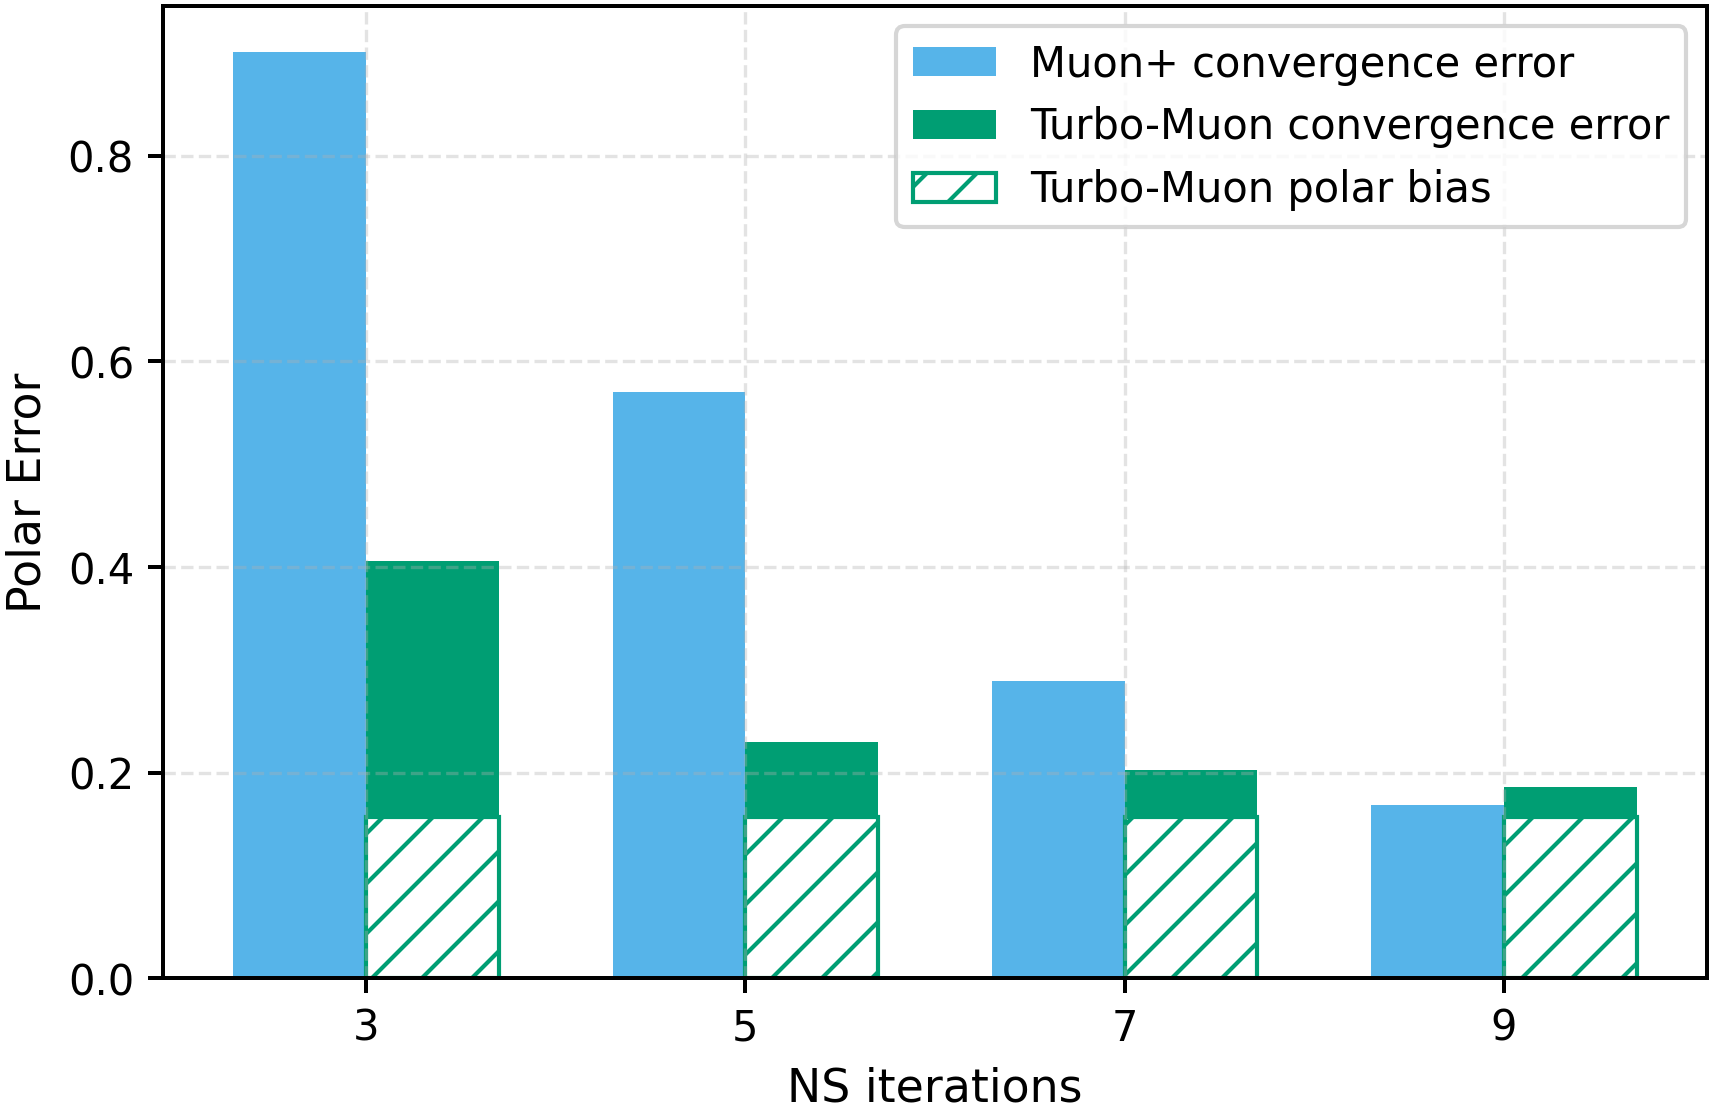
\includegraphics[width=\textwidth]{figures/ch5_turbo_muon/convergence/approximation_error_levy-1.0.png}
            \caption{Levy distribution: $\alpha = 1.0$, $\beta = 0$}
        \end{subfigure}
        \hfill
        \begin{subfigure}{0.32\textwidth}
            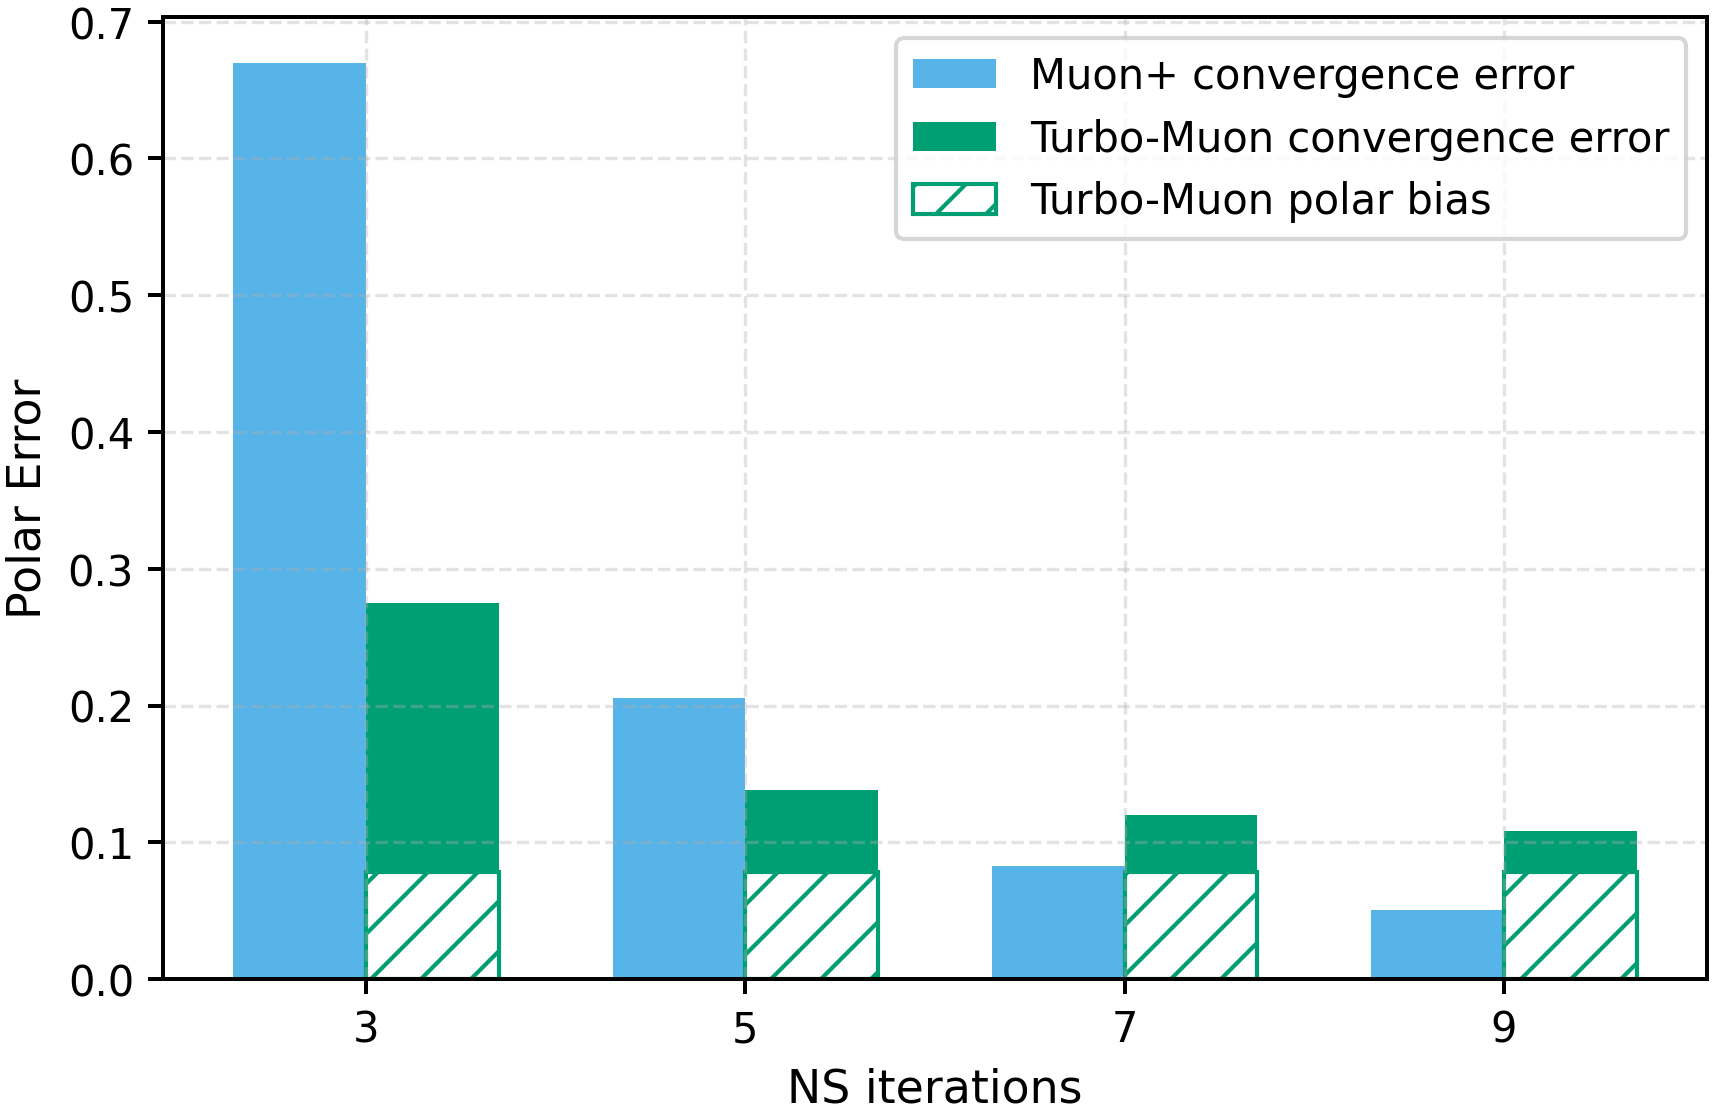
\includegraphics[width=\textwidth]{figures/ch5_turbo_muon/convergence/approximation_error_levy-1.5.png}
            \caption{Levy distribution: $\alpha = 1.5$, $\beta = 0$}
        \end{subfigure}
        \hfill
        \begin{subfigure}{0.32\textwidth}
            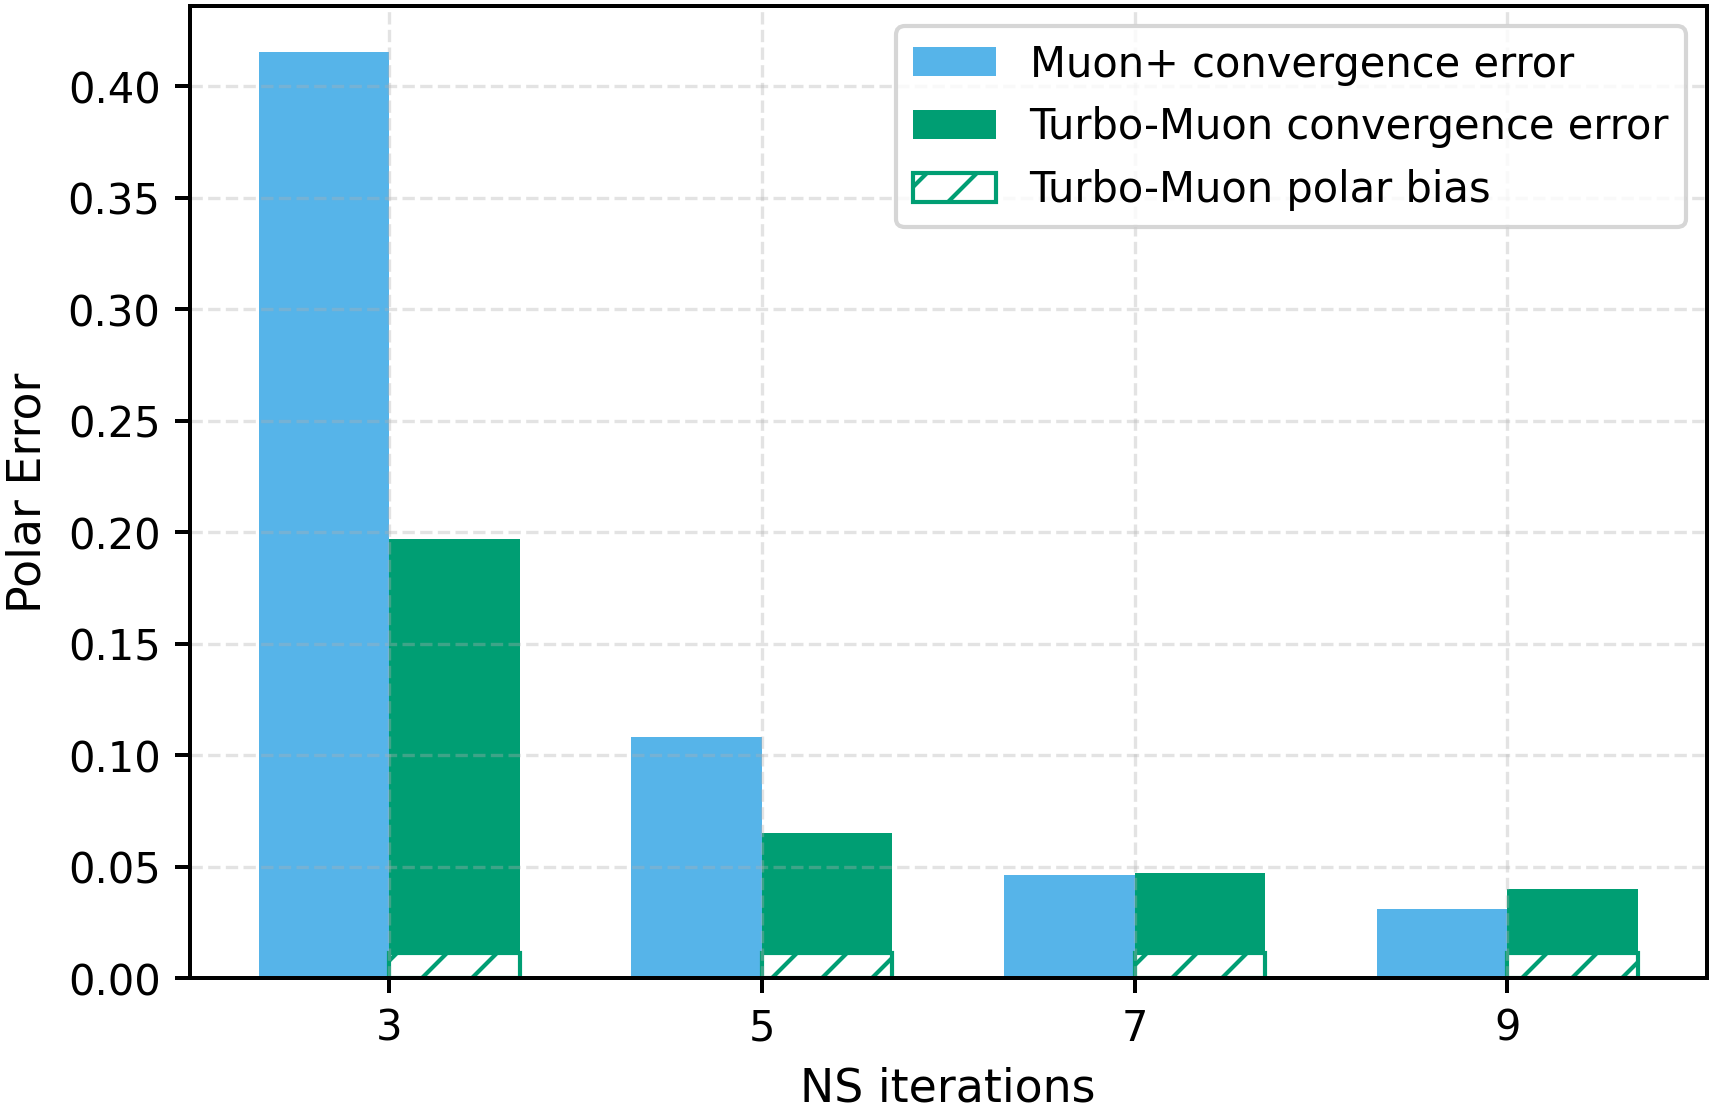
\includegraphics[width=\textwidth]{figures/ch5_turbo_muon/convergence/approximation_error_levy-2.0.png}
            \caption{Levy distribution: $\alpha = 2.0$, $\beta = 0$}
        \end{subfigure}
        \caption{Reproduction of \cref{fig:bias_converge} with heavy tailed distributions. This extreme regime--where the singular value decomposition is at its numerical limit-- shows that the tail index correlates with the bias error induced by our preconditioning.}
        \label{fig:bias_converge_levy}
    \end{figure*}
    
    Interestingly, in these regimes, the orthogonality error of \turbomuon is very low, highlighting that the remaining error is not due to a lack of convergence but to an increased bias for poorly conditioned matrices. This can be observed by reproducing the \cref{fig:bias_converge_levy} experiment from the paper: for instance, when $\alpha=1$, the polar bias can reach up to 0.15, which is significantly higher than the bias found with matrices sampled from normal distributions. Yet the drastically improved convergence still leads to a lower polar error compared to Muon+, which requires nine iterations (27 matrix multiplications) to reach a lower polar error than \turbomuon. The polar bias observed in \cref{tab:asymptotic} suggests that empirical gradients have a tail index $1.0 \leq \alpha \leq 1.5$, which is coherent with the observations of \cite{Simsekli2019TailIndex}.
    

\section{Result for various matrix sizes}
    \label{ap:more_normal_results}
    
    In this section, we show that the results displayed in \cref{fig:pareto8192} of the main paper hold for various matrix sizes sampled from the Normal distribution. Interestingly, two effects are observed: on one side, our preconditioning yields improvements in the polar error (shifting \turbomuon on the vertical axis), especially for large matrices; however, this effect becomes smaller for small matrices. On the other side, the triton kernel of 
    \cref{alg:muon} line 5
    %\cref{eq:ns_step_3} 
    improves runtime (shifting \turbomuon on the horizontal axis) on small matrices, as those lead to communication-bound kernels. Similarly, this effect becomes smaller for large matrices, as those lead to compute-bound kernels. This combination ensures a dominance of \turbomuon in all configurations.
    
    \begin{figure*}
        \centering
        
\includegraphics[width=0.32\textwidth]{figures/ch5_turbo_muon/plots_out/normal/bfloat16/pareto/pareto_size64.png}
        \hfill
        
\includegraphics[width=0.32\textwidth]{figures/ch5_turbo_muon/plots_out/normal/bfloat16/pareto/pareto_size256.png}
        \hfill
        
\includegraphics[width=0.32\textwidth]{figures/ch5_turbo_muon/plots_out/normal/bfloat16/pareto/pareto_size512.png}
        \hfill
        
        
\includegraphics[width=0.32\textwidth]{figures/ch5_turbo_muon/plots_out/normal/bfloat16/pareto/pareto_size1024.png}
        \hfill
        
\includegraphics[width=0.32\textwidth]{figures/ch5_turbo_muon/plots_out/normal/bfloat16/pareto/pareto_size2048.png}
        \hfill
        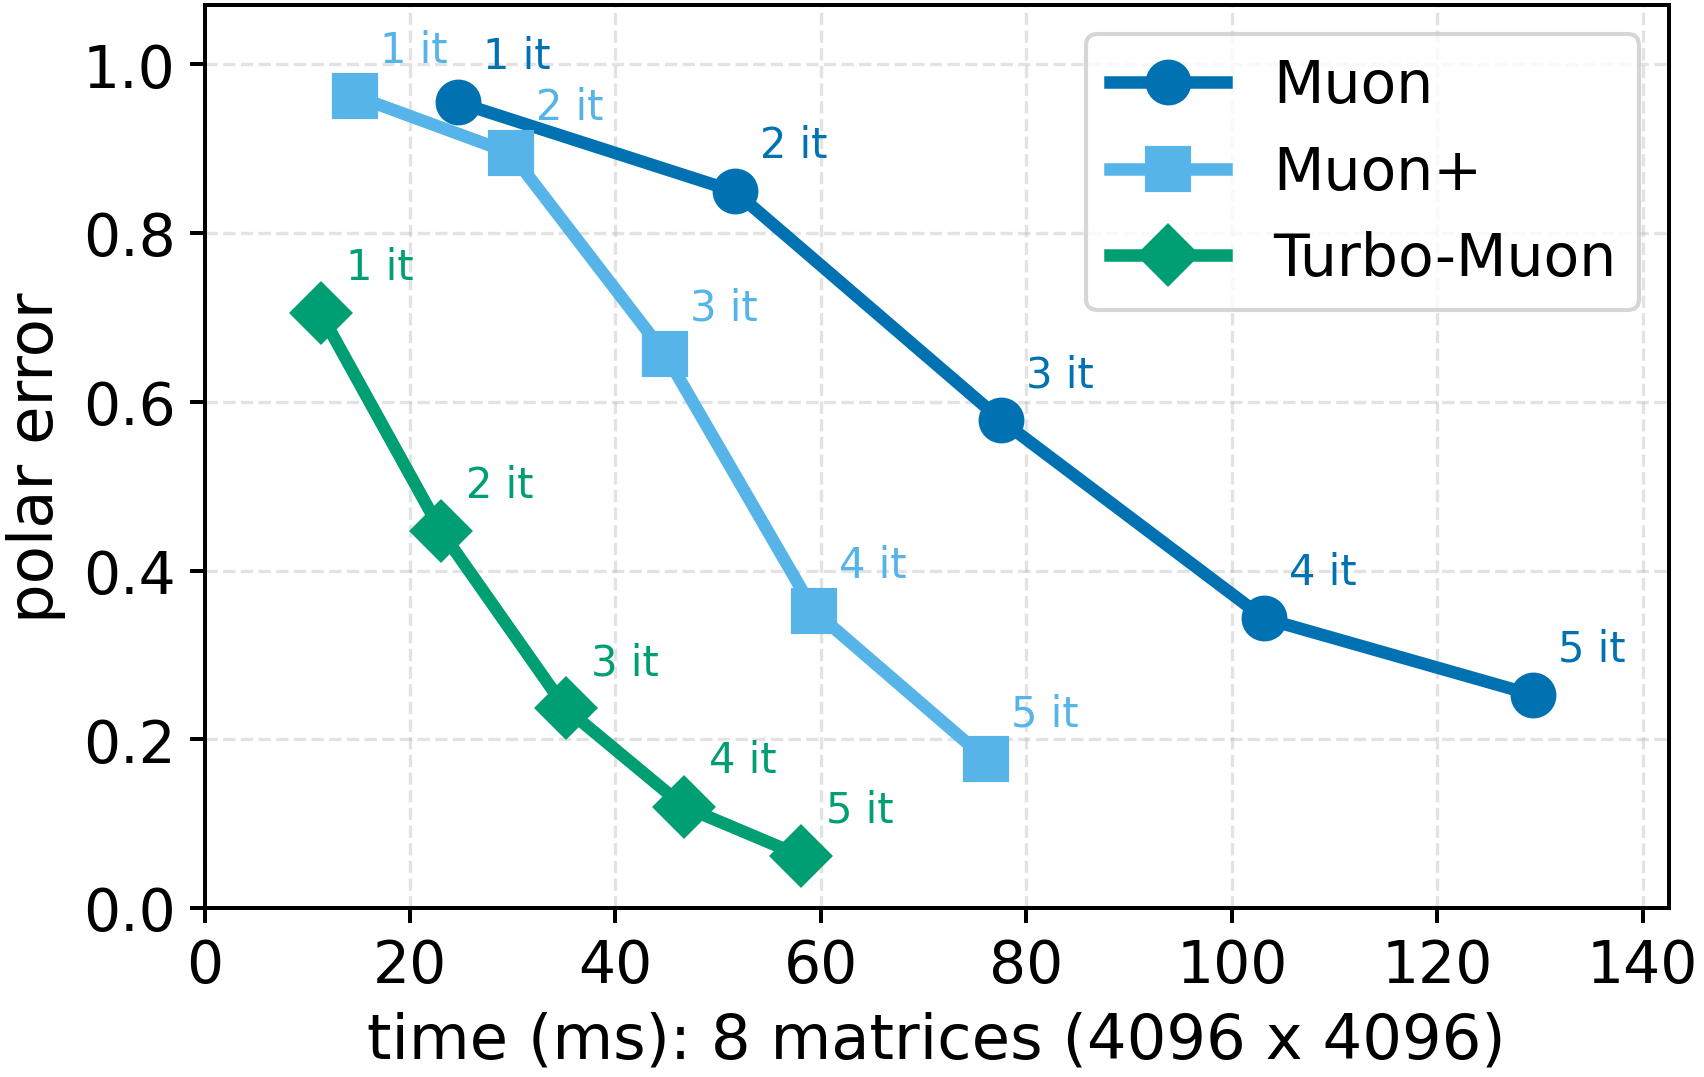
\includegraphics[width=0.32\textwidth]{figures/ch5_turbo_muon/plots_out/normal/bfloat16/pareto/pareto_size4096.png}
        
        \caption{Reproduction of \cref{fig:pareto8192} for various matrix sizes. In all settings, \turbomuon outperforms Muon and Muon+ by a significant margin.}
        \label{fig:pareto_all}
    \end{figure*}

\section{Comparison with other pre-conditioning strategies}
\label{ap:other_preconditioning}

AOL preconditioning is one possible way to improve the initialization of the Newton-Schulz iterations, but other normalization strategies may also be considered. As an additional baseline, we evaluate Schatten-$4$ normalization\cite{grishina_accelerating_2025}, which rescales a matrix $X$ by its Schatten-$4$ norm,
\[
    \|X\|_{S_4}
    =
    \left( \sum_i \sigma_i^4 \right)^{1/4}.
\]
This pre-conditioning can also be computed efficiently using the Frobenius norm of $A_0$ (\cref{alg:turbomuon} line~1). Unlike the Frobenius norm, this normalization gives more weight to larger singular values and can therefore provide a stronger control of the spectrum before applying Newton-Schulz.

The results are reported in \cref{fig:schatten4_size,fig:schatten4_iterations}. Schatten-$4$ normalization consistently improves over the standard Frobenius initialization used in Muon. However, AOL preconditioning remains better across matrix sizes and across Newton-Schulz iterations. In particular, AOL reaches lower polar error at each iteration, which is the relevant regime for Muon-style optimizers, where only a small number of Newton--Schulz steps is used in practice.


    \begin{figure*}
        \centering
        \begin{subfigure}{0.49\textwidth}
        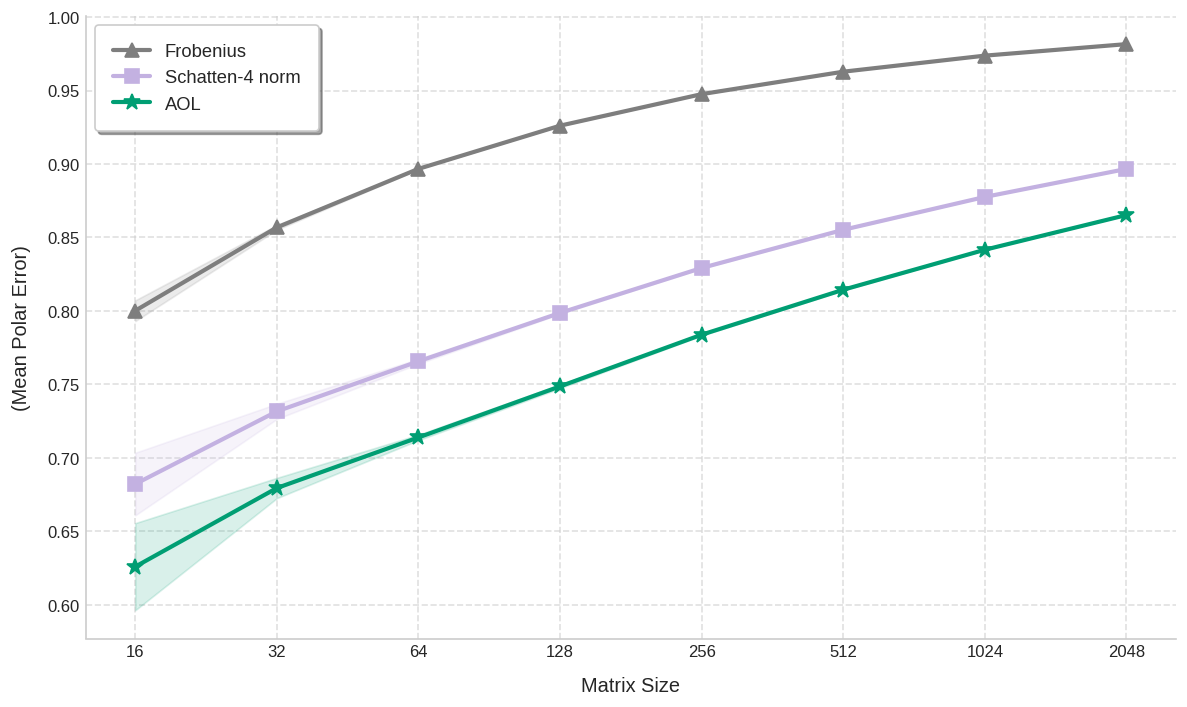
\includegraphics[width=\textwidth]{figures/ch5_turbo_muon/plots_out/normal/bfloat16/schatten4_comparison.png}
        \caption{Comparison of several pre-conditioning initializations}
        \label{fig:schatten4_size}
        \end{subfigure}
        \hfill
        \begin{subfigure}{0.49\textwidth}
        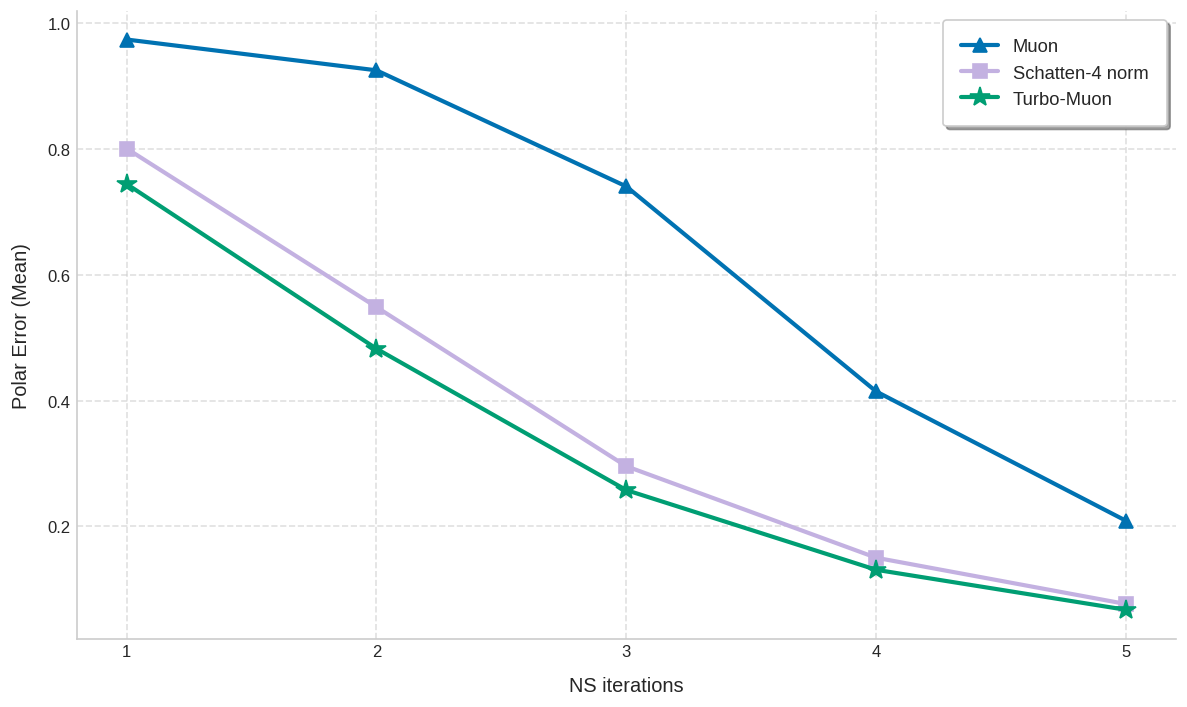
\includegraphics[width=\textwidth]{figures/ch5_turbo_muon/plots_out/normal/bfloat16/pareto/schatten4_comparison_NSIter.png}
        \caption{Comparison of Newton-Schulz across iterations with several pre-conditioning initialization}
        \label{fig:schatten4_iterations}
        \end{subfigure}
    \end{figure*}

%These experiments show that Turbo-Muon's improvement does not simply come from replacing Frobenius normalization by an arbitrary stronger normalization. Rather, the Gram-based, column-wise structure of AOL preconditioning appears to provide a more effective initialization than global norm-based alternatives such as Schatten-$4$ normalization.


\section{About the tuning of Newton-Schulz coefficients}
    \label{ap:polar_params}
    
    In this paper, we use dynamic polynomial coefficients to run Newton-Schulz iterations, which means that each step uses different values for $a, b, c$. However, the implementation of Muon+~\cite{ahn_dion_2025} uses coefficients computed explicitly for a fixed number of 5 iterations. To adapt the algorithm to a lower number of iterations, we employed a straightforward strategy as we reduced the number of iterations by retaining only the $n$ last polynomial coefficients. The motivation behind this choice was to isolate the effect of AOL preconditioning as the only factor responsible for the reduction in polar error between Muon+ and \turbomuon. 
    In this section, we demonstrate, through additional experiments, that our strategy is indeed highly effective in regimes with a low number of iterations.
    
    \subsection{Ablation }
    
    The difference between Muon and Muon+ shows the undeniable impact of using explicitly computed polynomial coefficients for a fixed number of steps. However, the improvement between the coefficients introduced by \cite{cesista2025muonoptcoeffs} and the coefficients introduced by \cite{amsel2025polar, grishina_accelerating_2025} is more nuanced, and is mainly observed on heavy-tailed distributions. Yet, the application of those polynomial coefficients to \turbomuon yields a negative impact. We hypothesize the root cause to be due to the assumption about the minimum singular value, required to compute the coefficients. Therefore, we leave the computation of optimal coefficients for \turbomuon as potential future work.
    
    \begin{figure*}[htbp]
        \centering
        \begin{subfigure}{0.32\textwidth}
            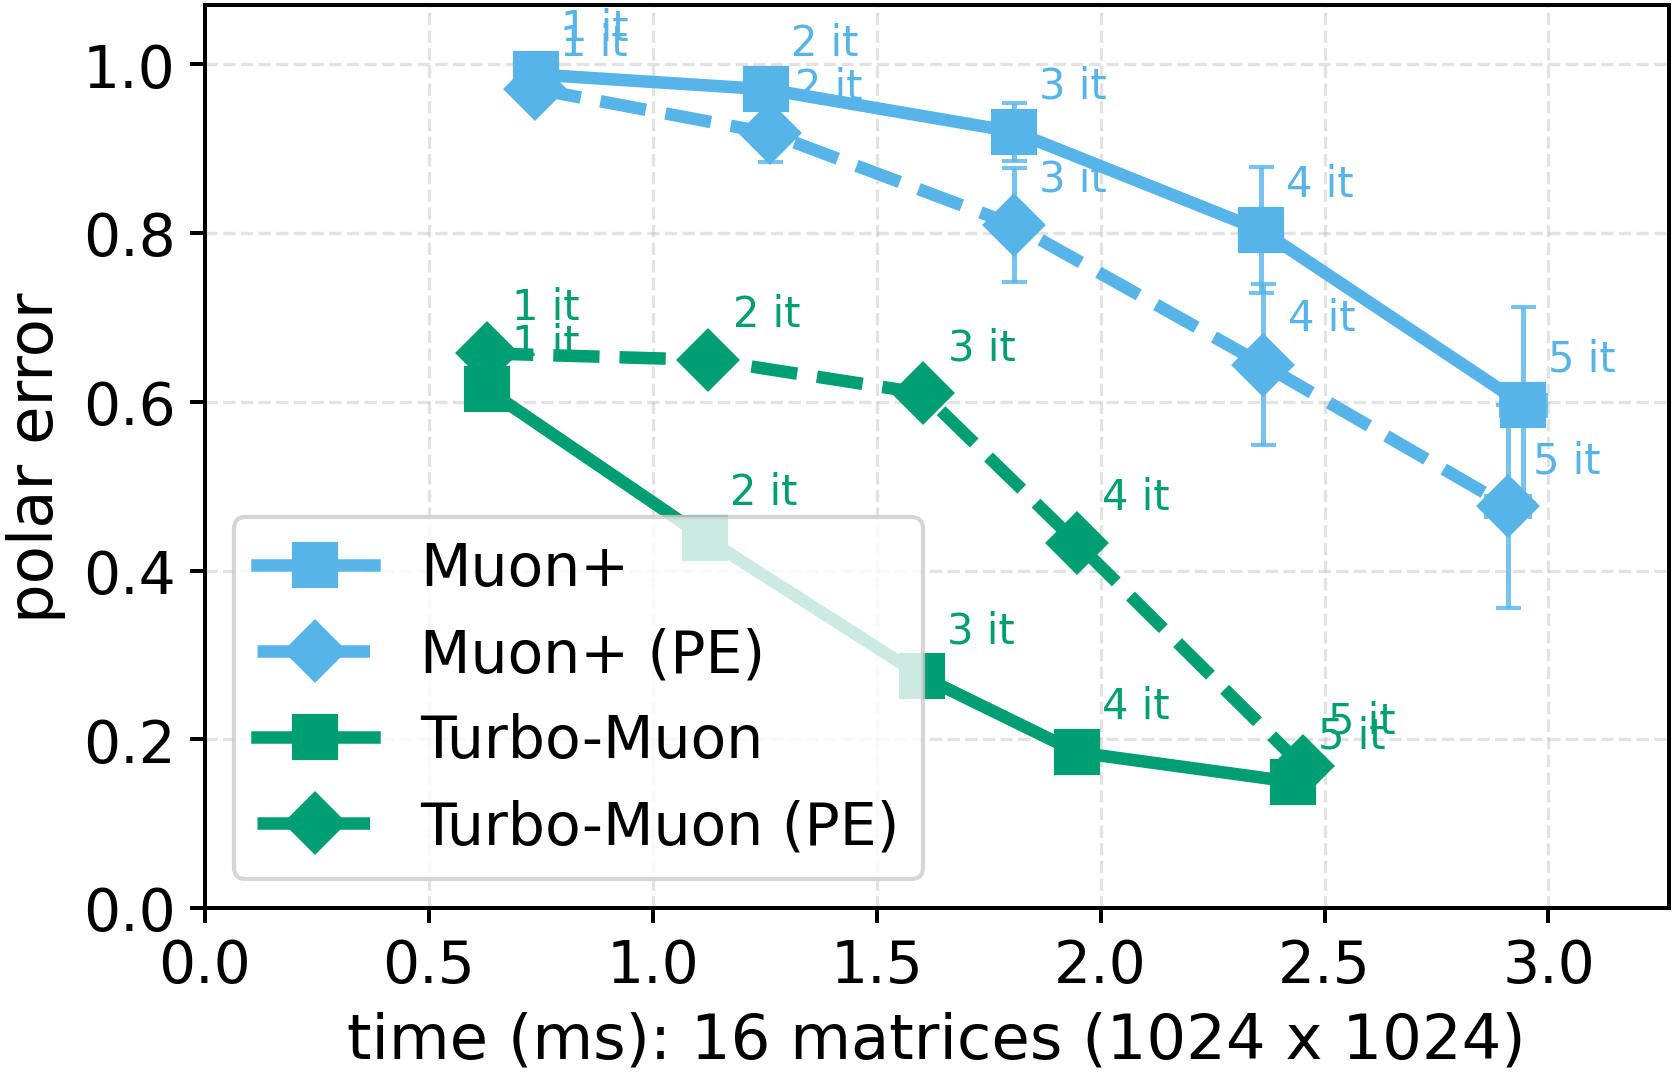
\includegraphics[width=\textwidth]{figures/ch5_turbo_muon/factors_analysis/plots_out/levy-1.0/bfloat16/pareto/pareto_size1024.png}
            \caption{Levy distribution: $\alpha = 1.0$, $\beta = 0$}
        \end{subfigure}
        \hfill
        \begin{subfigure}{0.32\textwidth}
            
\includegraphics[width=\textwidth]{figures/ch5_turbo_muon/factors_analysis/plots_out/levy-1.5/bfloat16/pareto/pareto_size1024.png}
            \caption{Levy distribution: $\alpha = 1.5$, $\beta = 0$}
        \end{subfigure}
        \hfill
        \begin{subfigure}{0.32\textwidth}
            
\includegraphics[width=\textwidth]{figures/ch5_turbo_muon/factors_analysis/plots_out/levy-2.0/bfloat16/pareto/pareto_size1024.png}
            \caption{Levy distribution: $\alpha = 2.0$, $\beta = 0$}
        \end{subfigure}
        
        \caption{Coefficients from \cite{amsel2025polar} are suboptimal when combined with AOL-preconditioning. We recomputed the optimal coefficient for each number of iterations, using default parameters ($l=10^{-3}$, $\text{cushion}=0.024$, and $\text{safety\_factor}=2\times10^{-2}$). For both Muon+ and \turbomuon, we report the performance using Polar Express (PE) and compare it with the original. On heavy-tailed distributions, these coefficients improve the performance of Muon+ but degrade the performance of \turbomuon.}
        \label{fig:polar_epxress_ablation}
    \end{figure*}
    

%\section{Direct comparison with nanoGPT fastest training procedure}
%\label{ap:nanogpt-WR}
\section{NanoGPT Speed-Run Details}
\label{ap:nanogpt-WR}

We adopt the Modded-NanoGPT benchmark~\cite{modded_nanogpt_2024}, a highly optimized training setup for a 124M-parameter GPT model on the FineWeb dataset~\cite{penedo2024fineweb}. The goal is to reach a validation cross-entropy of 3.28, corresponding to the estimated performance of GPT-2~\cite{radford2019language}, in minimal wall-clock time. The reference performance is in less than 3 minutes on 8×NVIDIA H100, consuming roughly 0.73B tokens.
This benchmark combines multiple architectural, optimization, and systems-level improvements, including rotary embeddings, QK normalization, ReLU\textsuperscript{2} activations, sliding-window and flash attention, an FP8 language modeling head, and the Muon optimizer. These optimizations are specifically designed to minimize training time and reduce optimizer overhead, making this setting particularly challenging for methods targeting further efficiency gains. Additionally, it places a strong emphasis on reproducible runtime measurement, enabling us to precisely evaluate whether our approach can also yield performance gains in end-to-end training even in highly efficient settings. 
\paragraph{Experimental protocol.} We reuse the most recent public training recipe and modify only the optimizer by replacing Muon with \turbomuon. The number of Newton--Schulz iterations is treated as a configurable parameter, while all other hyperparameters (learning rate, batch size, architecture, and data pipeline) are kept unchanged.
All experiments are conducted on 4$\times$ NVIDIA H100 GPUs. For each configuration, we report the average validation loss and runtime over 10 independent runs to account for runtime variability.
\paragraph{Results.}
As reported in \cref{tab:nanoGPT_accuracy}, \turbomuon achieves equivalent validation performance while requiring one fewer Newton--Schulz iteration. This reduction translates into a consistent decrease in total runtime. In particular, \cref{tab:end2endperf} shows a reduction from $274.75 \pm 0.14$ seconds for the fastest Muon+ configuration to $266.00 \pm 0.10$ seconds when using \turbomuon.

%\paragraph{Discussion.}
%This benchmark is deliberately optimized to minimize the relative cost of the Muon optimizer, making it a conservative setting for evaluating improvements in the orthogonalization step. Despite this, \turbomuon consistently provides measurable runtime gains without requiring any hyperparameter tuning.

%\paragraph{Additional analyses.}
%We further investigate the impact of \turbomuon under different training regimes in \cref{ap:trainingregimes}, including variations in batch size and model scale, to better characterize the regimes in which the proposed method yields the largest benefits.

\paragraph{Additional analyses.}
    While the experiment depicted in \cref{tab:nanoGPT_accuracy} compared Muon, Muon+, and \turbomuon, we noted that the nano-GPT speedrun script used the implementation of Muon+ with a different set of NS coefficients from \cite{amsel2025polar, grishina_accelerating_2025} (Depicted as Muon+ (PE) in \cref{ap:polar_params}). Given the additional insights of the experiments of \cref{ap:polar_params}, this choice could be seen as biased in favor of Turbo-Muon. To alleviate any doubts, we reproduced this experiment using the Polar Express factors tested in \cref{ap:polar_params}, which would favor the baseline over \turbomuon.


    In this setting, we compare \turbomuon (PE) with \textbf{four} iterations with Muon+ (PE) with \textbf{five} iterations. In order to remove one iteration, we applied the same strategy that was used between Muon+ and \turbomuon{}, which is discussed in \cref{ap:polar_params}. In order to run this training on 4xH100 instead of 8, we used a gradient accumulation of 2 to match the original results.
    We performed 10 trials in a row in order to measure variance on the final validation loss and the total runtime. This was done for both the baseline and our improved version to obtain comparable results. 

    \begin{table*}[htbp]
        \centering
        \begin{tabular}{llrrrr}
        \toprule
         method & iterations & val loss  & val loss std & runtime & runtime std \\
        \midrule
        Muon+ (PE) & 5it & 3.2774 & 0.0014 & 273.75s & 0.14 \\
        \turbomuon (PE) & 4it & 3.2791 & 0.0013 & 266.65s & 0.10 \\
        \bottomrule
        \end{tabular}
        \caption{Direct comparison against the original training procedure. Results reported for 10 trials for each variant.}
        \label{tab:wr_comp}
    \end{table*}

    Interestingly, we can observe a degradation of only $0.0017$ in the final loss. These results can be observed through the lenses of observations made in \cref{ap:polar_params}: where we observed that factors obtained from \cite{amsel2025polar, grishina_accelerating_2025} underperformed when combined with AOL preconditioning. However, this degradation is smaller than the degradation observed when removing one iteration as done in \cref{tab:nanoGPT_accuracy}.

    
%\section{Runtime improvements for medium-scale training}
\section{Runtime influence of the training regime}
\label{ap:trainingregimes}
In practice, the optimizer step accounts for only a small fraction of total training computational cost, which is usually dominated by forward and backward propagation. Nonetheless, Muon’s orthogonalization introduces a measurable overhead compared to AdamW. This overhead decreases as the batch size increases, since Muon’s computational cost is independent of the batch dimension, while the model’s forward cost scales linearly with it. Larger batches, therefore, improve time-to-target performance and typically move Muon past AdamW on the compute-efficiency frontier \cite{shah2025practical}, especially as Muon exhibits a larger critical batch size\cite{wen_fantastic_2025}.


\begin{table*}[t]
    %\begin{subfigure}[b]{0.49\textwidth}
        \centering
        \begin{tabular}{lcc}
        \hline
        \textbf{Variant} & \textbf{ms/step} & \textbf{Speedup} \\
        \hline
        \multicolumn{3}{c}{\textbf{Muon variants}} \\
        \hline
        \color{muoncolor}Muon   & $1378.54 \pm 12.35$ & 1.000x \\
        \color{dioncolor}Muon+   & $1308.09 \pm 8.36$  & 1.054x \\
        \color{turbomuoncolor}\turbomuon   & $1261.93 \pm 6.89$  & 1.092x \\
        \hline
        \multicolumn{3}{c}{\textbf{Dion (Muon-derived, large-scale oriented)}} \\
        \hline
        dion-1          & $3477.93 \pm 57.22$ & 0.397x \\
        dion-1/4        & $1678.71 \pm 14.64$ & 0.821x \\
        dion-1/16       & $1229.01 \pm 14.55$ & 1.122x \\
        \hline
        \end{tabular}
        \vspace{1mm}
        \caption{
        \textbf{Turbo-Muon unlocks step-time speedups at medium scale.}
        We report training throughput (ms per optimization step) when simulating the training of a 1.3B-parameter model on an A100 80GB GPU with a batch size of 32k tokens per GPU, a setting where Muon's overhead is clearly exposed, and Dion's low-rank induces a perceptible loss degradation.
        The speedup column indicates performance relative to \texttt{Muon}, with higher values corresponding to faster training.
        }
        \label{tab:1b_runtime}
\iffalse
    \end{subfigure}
    \hfill
    \begin{subfigure}[b]{0.49\textwidth}
        \centering
        %\begin{tabular}{lll}
        %    \toprule
        %     \color{turbomuoncolor}\turbomuon & \color{dioncolor}Muon+ & \color{muoncolor}Muon \\
        %   \midrule
        %        3.35 ± 0.002 \color{turbomuoncolor}{(\textbf{1}it}) & 3.35 ± 0.003 (2it)& 3.34 ± 0.002 (2it) \\
        %        3.32 ± 0.001 \color{turbomuoncolor}{(\textbf{2}it}) & 3.31 ± 0.002 (3it)& 3.30 ± 0.002 (3it) \\
        %        3.29 ± 0.001 \color{turbomuoncolor}{(\textbf{3}it}) & 3.29 ± 0.003 (4it)& 3.29 ± 0.005 (4it) \\
        %        3.28 ± 0.001 \color{turbomuoncolor}{(\textbf{4}it}) & 3.28 ± 0.003 (5it)& 3.28 ± 0.001 (5it) \\
        %    \bottomrule
        %\end{tabular}
        \begin{tabular}{p{1mm} lll}
        \toprule
        \textbf{It} & \color{turbomuoncolor}\turbomuon & \color{dioncolor}Muon+ & \color{muoncolor}Muon \\
        \midrule
        
        % 2 
        % & \cellcolor{orange!80} 3.32$\pm 1e^{-3}$ 
        % & \cellcolor{red!80} 3.35$\pm 3e^{-3}$ 
        % & \cellcolor{red!73} 3.34$\pm 2e^{-3}$ \\
        
        % 3 
        % & \cellcolor{yellow!80} 3.29$\pm 1e^{-3}$ 
        % & \cellcolor{orange!73} 3.31$\pm 2e^{-3}$ 
        % & \cellcolor{orange!66} 3.30$\pm 2e^{-3}$ \\
        
        % 4 
        % & \cellcolor{green!80} 3.28$\pm 1e^{-3}$ 
        % & \cellcolor{yellow!80} 3.29$\pm 3e^{-3}$ 
        % & \cellcolor{yellow!80} 3.29$\pm 5e^{-3}$ \\
        
        % 5 
        % &  \cellcolor{green!80} 3.28$\pm 1e^{-3}$ 
        % & \cellcolor{green!80} 3.28$\pm 3e^{-3}$ 
        % & \cellcolor{green!80} 3.28$\pm 1e^{-3}$ \\

        2 
        & \cellcolor{red!15!white} 3.32$\pm 1e^{-3}$ 
        & \cellcolor{red!25!white} 3.35$\pm 3e^{-3}$ 
        & \cellcolor{red!20!white} 3.34$\pm 2e^{-3}$ \\
        
        3 
        & \cellcolor{red!10!blue!5} 3.29$\pm 1e^{-3}$ 
        & \cellcolor{red!12!white} 3.31$\pm 2e^{-3}$ 
        & \cellcolor{red!10!white} 3.30$\pm 2e^{-3}$ \\
        
        4 
        & \cellcolor{blue!12!white} 3.28$\pm 1e^{-3}$ 
        & \cellcolor{red!8!blue!8} 3.29$\pm 3e^{-3}$ 
        & \cellcolor{red!8!blue!8} 3.29$\pm 5e^{-3}$ \\
        
        5 
        & \cellcolor{blue!15!white} 3.28$\pm 1e^{-3}$ 
        & \cellcolor{blue!15!white} 3.28$\pm 3e^{-3}$ 
        & \cellcolor{blue!15!white} 3.28$\pm 1e^{-3}$ \\
        
        \bottomrule
        \end{tabular}
        \vspace{6mm}
        \caption{\textbf{Our approach allows the removal of one Newton-Schulz iteration:} We trained a 144M GPT model on the FineWeb dataset\cite{penedo2024fineweb} up to the performance of GPT-2 and reported validation loss. We reused the fastest existing training script and replaced the Newton-Schulz implementation without changing any other parameters. %Each line compared \turbomuon with baselines that have one extra iteration.
        }
        \label{tab:nanoGPT_accuracy}
        \vspace{3.5mm}
    \end{subfigure}
    \caption{\textbf{\turbomuon can make realistic training faster without impact on final loss.} \cref{tab:1b_runtime} shows that it can achieve non-negligible speedups on medium-scale training, with runtime improvements nearing 10\% of the total step runtime. \cref{tab:nanoGPT_accuracy} shows that our approach does not induce perceptible loss degradation when an iteration is removed.}
\fi
\end{table*}

\begin{figure*}[t]
    \centering
\end{figure*}

At large model scales, however, global batch size cannot grow indefinitely without sharding, which significantly affects compute efficiency. Naïve replication can increase per-step flops by up to 5×, while more advanced strategies such as sharded matrix multiplication or layer sharding can suffer from bandwidth saturation. The resulting trade-off is tightly linked to the per-device batch size, which limits the amortization of Muon’s overhead \cite{essential2025muon}, leading to an overhead typically around 10-20\%.

Within this context, our preconditioned Newton–Schulz method reduces the cost of the orthogonalization subroutine by approximately 3× at fixed polar accuracy. The resulting end-to-end gains are most pronounced at medium scales—where batch size is reduced but full sharding is unnecessary. This regime is illustrated in \cref{tab:1b_runtime}: On a 1.3B language model, one A100 with 80G memory can achieve a batch size of 32k tokens without sharding. In this context, Muon’s cost is non-negligible, but optimizers tailored for extreme scales, such as Dion\cite{ahn_dion_2025}, are not yet efficient: Dion's low-rank updates--which shine at larger scales--still degrade convergence. Our drop-in preconditioned NS offers a competitive trade-off by reducing computational cost without compromising accuracy.

\section{CIFAR-10 Speed-Run Details}
\label{ap:cifar}

\paragraph{Benchmark description.}
We consider the CIFAR-10 speed-running task~\cite{Jordan2024cifar10airbench}, which aims to reach 94\% validation accuracy on CIFAR-10~\cite{krizhevsky2009learning} in minimal wall-clock time on a single H100 GPU. Unlike NanoGPT, this benchmark involves training a convolutional neural network (CNN).

\paragraph{Optimizer behavior.}
In this setting, Muon reshapes convolutional gradient updates into matrices and applies iterative orthogonalization, providing a complementary regime to evaluate AOL preconditioning.

\paragraph{Results.}
\turbomuon achieves identical accuracy while reducing runtime from $1.359$ s to $1.348$ s, corresponding to a 0.81\% speedup (\cref{tab:end2endperf}).

\paragraph{Discussion.}
Although the absolute gain is modest due to the already optimized implementation, this result confirms that AOL preconditioning consistently improves efficiency across heterogeneous architectures and training setups.

\section{
On the complementarity of  \turbomuon with other Muon improvements
} \label{ap:tridao}

Concurrent with this work, \cite{GramNewtonSchulz} proposed a Gram-based, hardware-aware variant of Newton-Schulz orthogonalization that further reduces the cost of Muon updates. This approach is complementary to our preconditioning strategy, as it modifies the implementation of the Newton-Schulz iterations whereas AOL modifies their initialization. We therefore evaluate their combination in \cref{tab:tridao} evaluating the runtime and residual polar error after five iterations of Newton-Schulz, on random input matrices of size $2048\time 5464$. Gram Newton-Schulz substantially reduces runtime compared to the Muon+ implementation, but slightly increases the polar error. Adding AOL preconditioning recovers part of this loss in approximation quality, while incurring only a modest runtime overhead.

\begin{table}[h]
\centering
\caption{Runtime and polar error of Newton--Schulz variants.}
\label{tab:tridao}
\begin{tabular}{lcc}
\toprule
Variant & Time (ms) & Polar error \\
\midrule
%Standard NS (PyTorch)      & 36.134 & $1.741946{\times}10^{-2}$ \\
\textcolor{dioncolor}{Muon+}      & 26.031 & $1.7419{\times}10^{-2}$ \\
%Gram NS (PyTorch)          & 29.371 & $1.743914{\times}10^{-2}$ \\
Gram NS \cite{GramNewtonSchulz}          & 20.621 & $1.7438{\times}10^{-2}$ \\
%AOL Gram NS (PyTorch)      & 31.846 & $1.741788{\times}10^{-2}$ \\
\textcolor{turbomuoncolor}{Turbo-Muon} + Gram NS    & 22.717 & $1.7431{\times}10^{-2}$ \\
\bottomrule
\end{tabular}
\end{table}


\section{
Beyond Iterative Approximations: On the Asymptotic Behavior of \turbomuon
} \label{ap:bias_analysis}


\begin{figure}
    \centering
    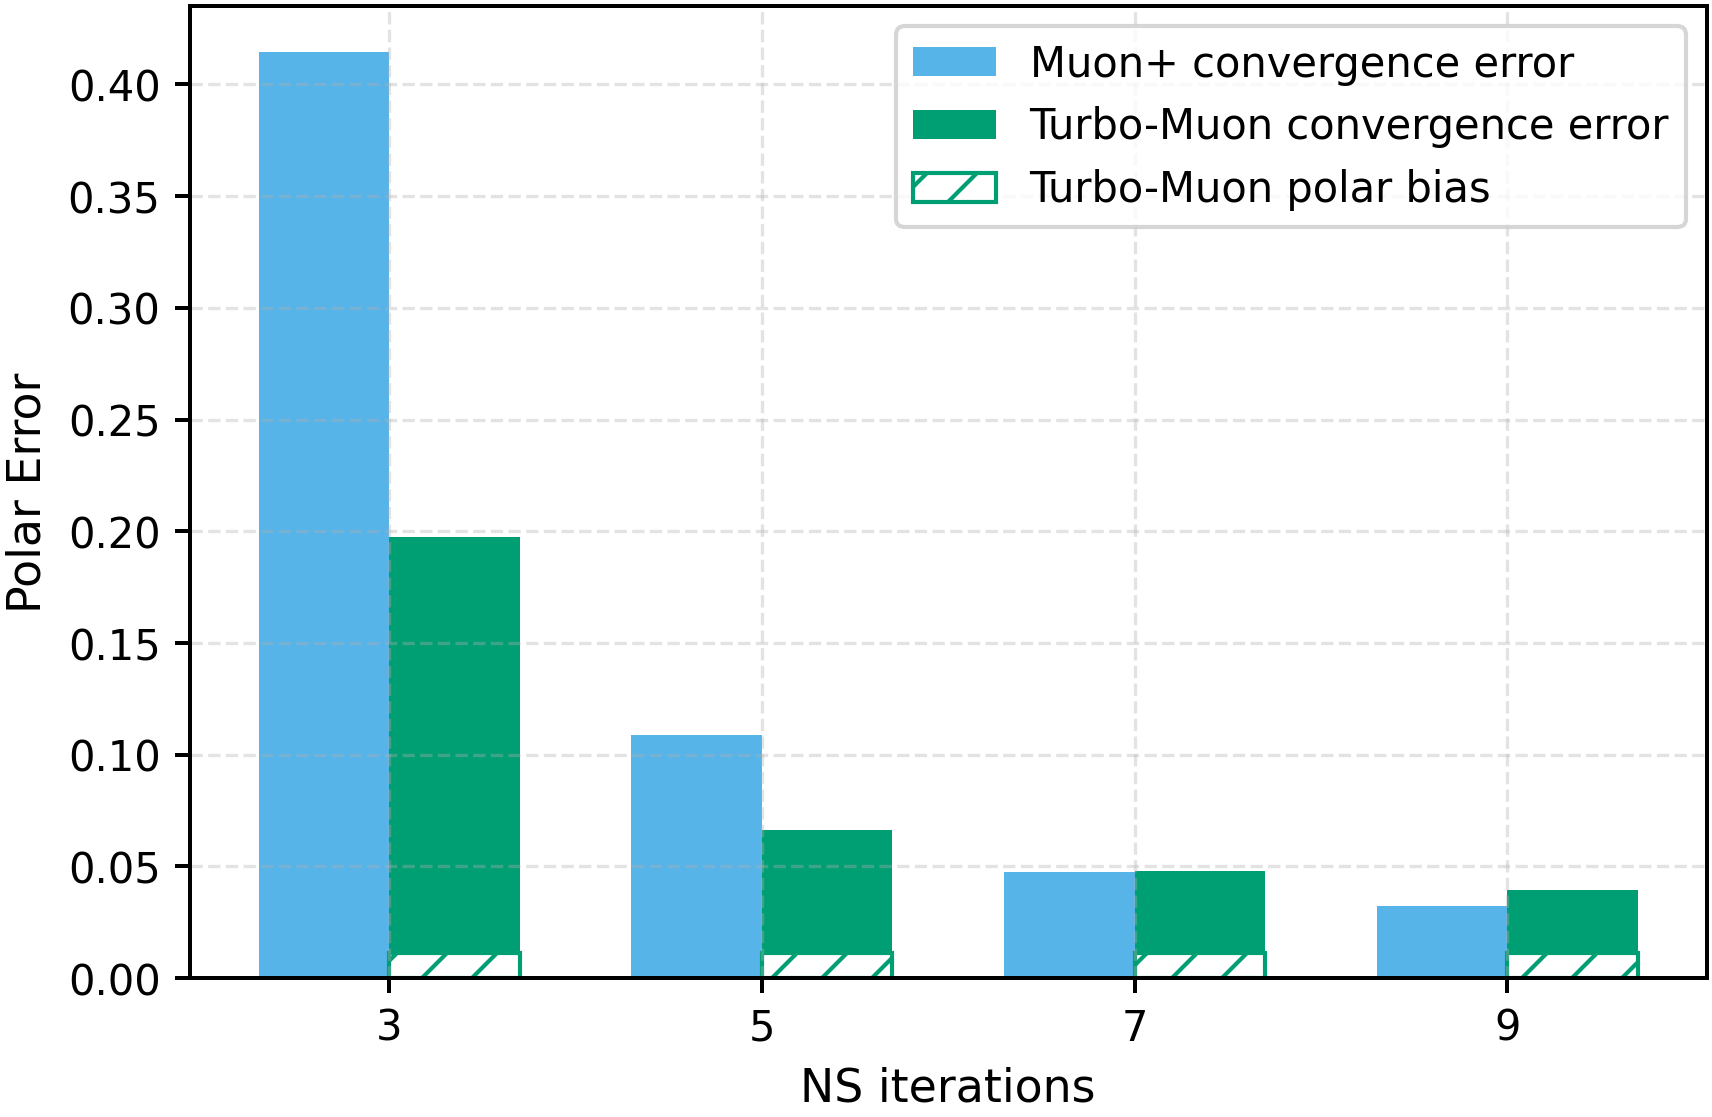
\includegraphics[width=0.45\linewidth]{figures/ch5_turbo_muon/convergence/approximation_error_normal.png}
    \caption{\textbf{Understanding the nature of the remaining polar error.} We decompose the polar error of the \turbomuon algorithm as an approximation error that depends on the number of NS iterations, along with a bias error that is introduced by AOL preconditioning. Results are measured on 100 random normal matrices.}
    \label{fig:bias_converge}
\end{figure}


In the previous sections, we have demonstrated that
$\varepsilon_{\text{polar}}(\operatorname{NS}_t\circ\textrm{AOL}, \mathbf{X}) \lessapprox \varepsilon_{\text{polar}}(\operatorname{NS}_t, \mathbf{X})$
in the widely adopted practical settings where $t \leq 5$. This means that the polar error is of the same order as the usual error made by approximation algorithms. 
However, the nature of this error remains to be determined: When does the remaining polar error come from a lack of orthogonality? or when does it come from a discrepancy between $\textrm{PolarFactor}(\textrm{AOL}(\mathbf{X}))$ and $\textrm{PolarFactor}(\mathbf{X})$ ? 
In the latter case, can this new type of error bias the global optimization process?
In this section, we quantify how AOL preconditioning can introduce a bias and prove that this eventual bias still yields a strict descent direction.

\paragraph{Characterizing the remaining polar error.}
We can quantify the bias error induced by AOL preconditioning, by computing precisely $\operatorname{PolarFactor}(X) = Q$ and $\operatorname{PolarFactor}(AOL(X)) = Q_{aol}$:
\[
    \varepsilon_{\text{bias}}(\mathrm{AOL}, \mathbf{X}) = \frac{\| \textbf{Q} - \textbf{Q}_{aol} \|_F}{\sqrt{n}}
\]
This can be interpreted as the irreducible error that cannot be reduced after full convergence of the Newton-Schulz algorithm with AOL preconditioning, since it converges toward $Q_{aol}$.
Similarly, we can define:
\[
    \varepsilon_{\text{approx}}(\operatorname{NS}_t, \textrm{AOL}(\mathbf{X})) = \frac{\|  \textbf{Q}_{aol} - \operatorname{NS}_t\circ\textrm{AOL}(\mathbf{X}) \|_F}{\sqrt{n}}
\]
Which represents the approximation error between $NS_t(AOL(X))$ and $Q_{aol}$.
These two definitions connect to the polar error with a direct application of the triangle inequality:
\[
    \varepsilon_{\text{polar}}(\operatorname{NS}_t\circ\textrm{AOL}, \mathbf{X}) \leq  
    \underbrace{\varepsilon_{\text{bias}}(\textrm{AOL}, \mathbf{X})}_{\text{irreducible bias}} + 
    \underbrace{\varepsilon_{\text{approx}}(\operatorname{NS}_t, \textrm{AOL}(\mathbf{X}))}_{\text{approximation error}}
\]

This allows us to view the approximation error of the polar factor of X by \turbomuon as a convergence-related error $\varepsilon_\text{approx}$ and a bias-related error $\varepsilon_\text{bias}$ term, which are dependent on the original matrix $\mathbf{X}$. Importantly, we assume that $\lim_{t\to\infty} \varepsilon_\text{approx}(\operatorname{NS}_t, \mathbf{X}) = 0$, as proven in ~\cite{bjorck1971iterative}. To illustrate this phenomenon, in \cref{fig:bias_converge}, we run an experiment where we orthogonalize the same batch of 100 random matrices using Newton-Schulz iterative steps. Since existing methods had coefficients computed for only five iterations, we recomputed those using the method from~\cite{amsel2025polar}. 
For each number of iterations, we quantify $\varepsilon_{\text{bias}}(\textrm{AOL}, \mathbf{X})$ (in dashed green) alongside $\varepsilon_{\text{approx}}(\operatorname{NS}_t, \textrm{AOL}(\mathbf{X}))$ (in dark green), finally, total polar error is compared with the polar error obtained without preconditioning, assuming that Newton-Schulz is perfectly unbiased (in dark blue).
We observe that while \turbomuon is indeed biased, its bias is compensated by the superior approximation speed it confers in practically adopted low $t$ settings. When $t$ is high, the beneficial effects of preconditioning are absorbed while the bias remains. For reference, nine iterations of Newton-Schulz require 27 matrix multiplications in total.


\paragraph{Characterizing AOL preconditioning when $t \rightarrow \infty$.}
We have shown that the bias effect is negligible in the low iteration number of Newton-Schulz usually used in Muon. But we might want to evaluate the effect it could induce in regimes where a high number of Newton-Schulz iterative steps are used. We show that in fact the biased estimation of the polar factor introduced by AOL preconditioning still ensures that we recover a weight update that corresponds to a steepest descent direction. For reference, as explained in~\cite{bernstein2024oldoptimizernewnorm}, 
%we have that 
the steepest descent update in spectral norm is (informally) defined as:
\vspace{1mm}
\begin{equation}
    \arg \min_{\Delta W} \left[ \langle G, \Delta W \rangle + \frac{\lambda}{2} \| \Delta W \|_2^2 \right] = \operatorname{PolarFactor}(G).
\label{eq:spectral_descent}
\end{equation}
\vspace{1mm}

\noindent with $G$ the gradient and $\lambda$ sharpness. Therefore, given that AOL preconditioning can be written as $\operatorname{AOL}(\mathbf{X}) = \mathbf{X}s$ with $s$ as vector with $s_i > 0$,  using Equation~\ref{eq:aol}. We have that the \turbomuon update solves a steepest descent in an induced norm that is dependent of $s$ (c.f. Definition 1 of \cite{bernstein2024oldoptimizernewnorm}).
Moreover, in practice, $s$ forms a vector of strictly positive entries. Therefore, \textit{the weight updates of \turbomuon yield a strict descent direction}. This means that even the worst case of an input that maximizes $\varepsilon_{\text{bias}}$ cannot lead to a divergence of the training process. More details are provided in Appendix~\ref{supp:descent_proof}.


\begin{table}[t]
    \vspace{1mm}
    \centering
    \label{tab:ns-aol}
    \begin{tabular}{cccccc}
    \toprule
    Method & $t_{\text{NS}}$ & Accuracy (\%) & $\varepsilon_\mathrm{approx}$ & $\varepsilon_\mathrm{bias}$ \\
    \midrule
    \turbomuon & 15 & $94.08 \pm 0.1 \%$ & $5.5 \times 10^{-4}$ & $0.1$ \\
    \turbomuon & 25 & $94.07 \pm 0.1 \%$ & $3.6 \times 10^{-4}$ & $0.1$ \\
    \turbomuon & 40 & $ 94.05 \pm 0.1 \%$ & $ 2.1 \times 10^{-4} $ & $0.1$ \\
    \midrule
    Muon & 15 & $94.06 \pm 0.1 \%$ & $1.5 \times 10^{-2}$ & $0.0$ \\
    Muon & 25 & $ 94.06 \pm 0.1 \%$ & $ 1.1 \times 10^{-2} $ & $0.0$ \\
    Muon & 40 & $ 94.04 \pm 0.1 \%$ & $ 7.4 \times 10^{-3} $ & $0.0$ \\
    \bottomrule
    \end{tabular}
    \caption{\textbf{The measured $\varepsilon_\mathrm{bias}$ does not impact final performance:} We measure  the final accuracy (\%) of the trained classifier on the CIFAR-10 dataset with and without AOL preconditioning after $t_{\text{NS}}$ steps. We log the values of $\varepsilon_\mathrm{approx}$ and $\varepsilon_\mathrm{bias}$ once every 10 train batches and report average values across 80 training runs.}
    \label{tab:asymptotic}
\end{table}

\paragraph{Confirming That the Estimation Bias Does Not Affect Training}
In order to empirically validate the theoretical result asserting that this estimation bias should not alter the training convergence, we investigate the training dynamics for an unconventionally high number of Newton-Schulz iterative steps.
We train a neural network on the CIFAR-10 dataset with and without AOL preconditioning. Across each run, we vary the number of iterative NS steps and compute coefficients for the NS iterations according to the number of chosen steps (using the method from~\cite{amsel2025polar}). The high number of steps we choose here leads to an unrealistically long training time, but ensures that the orthogonalized weight updates are extremely close estimates of $\operatorname{PolarFactor}(\mathbf{X})$ and $\operatorname{PolarFactor}(\operatorname{AOL}(\mathbf{X}))$.
Table~\ref{tab:asymptotic} depicts the results for $15\leq t_\mathrm{NS} \leq 40$, and shows that while both \turbomuon and Muon converge toward their respective iterative objective, the bias induced by the AOL-preconditioning has no impact on the quality of training.

%While it is unclear if AOL preconditioning confers an advantage in high $t$ regimes. 
Since we have shown in \cref{sec:steepest} that \turbomuon yields steepest descent
directions in an induced norm based on $\operatorname{PolarFactor}(GS)$, 
%It is rather apparent than 
training a neural network with \turbomuon's weight updates is valid in theory and in practice. Furthermore, usual practical implementations of orthogonality-based optimization rely on a relatively small amount of iterative steps to retrieve an approximation of the closest orthogonal matrix, where AOL preconditioning really shines.

